\documentclass[a4paper]{article}

\usepackage[english]{babel}
\usepackage[utf8x]{inputenc}
\usepackage{amsmath}
\usepackage{graphicx}
\usepackage[colorinlistoftodos]{todonotes}

\usepackage{listings}
\lstset{
	language=Python,
	backgroundcolor=\color{white},
	breaklines=true,
	%prebreak={\carriagereturn},
 	breakautoindent=true,
 	numbers=left,
 	numberstyle=\tiny,
 	stepnumber=2,
 	numbersep=5pt,
 	keywordstyle=\color{blue},
   	commentstyle=\color{green},
   	stringstyle=\color{gray},
	captionpos=b,
	frame=single,
	basicstyle=\footnotesize
}

\usepackage{setspace}
\onehalfspacing

\usepackage{csquotes}

\setlength{\parindent}{0pt}

\title{Advanced Mathematics for Engineers - Laboratory Problems}
\author{Eric Saier (eric.saier@hs-weingarten.de)\\Mat-Nr. 28224}

\begin{document}
\maketitle


%\mainmatter

\section{Linear Algebra}

First of all, a function to properly print vectors and matrices could come in handy. This can be realized the following way:

\begin{lstlisting}[caption=Functions to properly print vectors and matrices]
def getNumberString(pNumber, strLength):
	nStr = str(round(pNumber, 2));
	
	if pNumber >= 0: nStr = " " + nStr;
	
	spacesBefore = strLength - len(nStr);
	
	if spacesBefore > 0:
		for i in range(spacesBefore): nStr = " " + nStr;
	
	return nStr;

def printVector(pVector):
    for element in pVector:
		print(getNumberString(element, 7));

def printMatrix(pMatrix):
	for row in pMatrix:
		rowStr = "";
		for element in row:
			rowStr += getNumberString(element, 7) + " ";
		print(rowStr);
\end{lstlisting}


\subsection{Problem 1.1}


\begin{figure}[!ht]
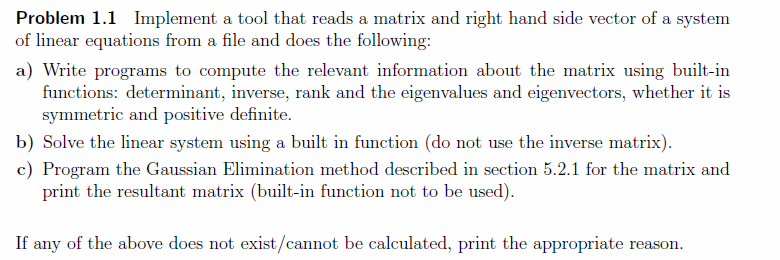
\includegraphics[width=1\textwidth]{chapters/images/desc-1-1}
\end{figure}


To read a matrix and a vector from a text file, first a form has to be determined, for example like this:

\begin{lstlisting}
1 -2 3 -4;
4.1 3 1.1 1;
2 4 1 4;
3 4 3 8;
####
6.1 5.2 4.2 3.1;
\end{lstlisting}

The first part is the matrix, where each line represents one row and each element within that row is seperated by a space. After a line of at least one hashtag, the following values are the elements of the vector, again seperated by a single space. If that form is adhered to, the matrix and vector can be read from the text file with the following script:

\begin{lstlisting}[caption=Extracting the matrix and vector from the text file]
def getVectorFromLine(line):
	numbers = [];
	numberString = "";
	for c in line:
		if c == ' ' or c == ';':
			numbers.append(float(numberString));
			numberString = "";
		else:
			numberString += c;
	
	return numbers;

myMatrix = [];
myVector = [];

textFile = open('matrixTextFile.txt', 'r');

readMatrix = True;

for line in textFile:
	if len(line) > 0:
		if line[0] == '#':
			readMatrix = False;
		else:
			vectorRead = getVectorFromLine(line);
			
			if readMatrix: myMatrix.append(vectorRead);
			else: myVector = vectorRead;


print("Matrix from file:");
mylib.printMatrix(myMatrix);

print("Vector from file:");
mylib.printVector(myVector);
\end{lstlisting}

Afterwards, the matrix and vector from the text file can be used as Python arrays, where the vector is a one-dimensional array and the matrix a two-dimensional array, with the single rows in the first dimension.


\subsubsection{a)}

For the built-in functions the Python library \textit{numpy} can be used:

\begin{lstlisting}[caption=Problem 1.1 a)]
import numpy as np;

matrixRows = len(myMatrix);
matrixCols = len(myMatrix[0]);
vectorRows = len(myVector);

isMatrixSquare = matrixRows == matrixCols;
notSquareStr = "matrix is not square";

matrixArr = np.array(myMatrix);
vectorArr = np.array(myVector);

print("determinant:");

if isMatrixSquare:
	detA = np.linalg.det(matrixArr);
	print(detA);
else:
	print(notSquareStr);

print("inverse:");

if isMatrixSquare:
	invA = np.linalg.inv(matrixArr);
	mylib.printMatrix(invA);
else:
	print(notSquareStr);

print("rank:");

rankA = np.linalg.matrix_rank(matrixArr);
print(rankA);

eigenValues = [];
eigenVectors = [];

if isMatrixSquare:
	eigA = np.linalg.eig(matrixArr);
	for eigi in eigA:
		for el in eigi:
			if isinstance(el, np.ndarray):
				eigenVectors.append(el);
			else:
				eigenValues.append(el);
	
	
	print("eigenvalues:");

	for eigenValue in eigenValues:
		print(eigenValue.real);

	print("eigenvectors:");

	for eigenVector in eigenVectors:
		print(eigenVector.real);
	
else:
	print("eigenvalues and eigenvectors");
	print(notSquareStr);

print("is symmetric:");

if isMatrixSquare:
	isSym = (matrixArr.transpose() == matrixArr).all();
	print(isSym);
else:
	print(notSquareStr);

print("is positive definite:");

if isMatrixSquare:
	isPosDef = np.all(np.linalg.eigvals(matrixArr));
	print(isPosDef);
else:
	print(notSquareStr);
\end{lstlisting}

The results are:

\begin{lstlisting}[caption=Result of 1.1 a), keywordstyle=\color{black}]
determinant:
169.2

inverse:
  -0.13    0.43   -0.53    0.15
   0.11   -0.17    0.71   -0.28
   0.29   -0.24     0.3    0.03
  -0.11    0.01   -0.26     0.2

rank:
4

eigenvalues:
8.25668694865
5.18909337619
-0.222890162424
-0.222890162424

eigenvectors:
[-0.31568286  0.44289131  0.61685718  0.61685718]
[ -7.86684467e-05   3.70103040e-01  -4.34768294e-01  -4.34768294e-01]
[ 0.38980754 -0.19285648 -0.40093074 -0.40093074]
[ 0.86509792 -0.79352215  0.10527324  0.10527324]

is symmetric:
False

is positive definite:
True
\end{lstlisting}

Since the matrix in the text file is square all calculations could be done.


\subsubsection{b)}

In order to solve the linear system, it has to be check first whether number of columns in the matrix equals the number of rows in the vector. If so, a built-in function from \textit{numpy} can be used to solve the system:

\begin{lstlisting}[caption=Problem 1.1 b)]
if not isMatrixSquare:
	print(notSquareStr);
	sys.exit();

if matrixCols != vectorRows:
	print("number of matrix columns and vector rows aren't equal");
	sys.exit();

linSolutions = np.linalg.solve(matrixArr, vectorArr);

xNum = 1;

for linSolution in linSolutions:
	print("x" + str(xNum) + " = " + str(linSolution));
	xNum += 1;
\end{lstlisting}

The resulting x values are:

\begin{lstlisting}[caption=Result of 1.1 b), keywordstyle=\color{black}]
x1 = -0.33829787234
x2 = 1.88156028369
x3 = 1.88794326241
x4 = -1.13439716312
\end{lstlisting}


\subsubsection{c)}

The Gaussian Elemination can be realized without an built-in function in the following way:

\begin{lstlisting}[caption=Problem 1.1 c)]
def gaussElemMethod(matrix, vector):
	n = len(matrix[0]);
	
	for k in range(n - 1):
		maxL = -1;
		for l in range(k, n):
			maxL = max(maxL, abs(matrix[l][k]));
		
		mFound = -1;
		
		for m in range(n):
			if abs(matrix[m][k]) == maxL:
				mFound = m;
		
		if mFound > 0 and matrix[mFound][k] == 0:
			print("singular");
			continue;
		
		for i in range(k + 1, n):
			qik = matrix[i][k] / matrix[k][k];
			
			for j in range(0, n):
				matrix[i][j] = matrix[i][j] - qik * matrix[k][j];
			
			vector[i] = vector[i] - qik * vector[k];

gaussElemMethod(myMatrix, myVector);

print("matrix after elimination:");
mylib.printMatrix(myMatrix);

print("vector after elimination:");
mylib.printVector(myVector);
\end{lstlisting}

Applying this function to the matrix and vector from the text file leads to the following results:

\begin{lstlisting}[caption=Result of 1.1 c), keywordstyle=\color{black}]
matrix after elimination:
    1.0    -2.0     3.0    -4.0
    0.0    11.2   -11.2    17.4
    0.0     0.0     3.0   -0.43
    0.0     0.0     0.0    5.04

vector after elimination:
    6.1
 -19.81
   6.15
  -5.71
\end{lstlisting}


\subsection{Problem 1.2}

\begin{figure}[!ht]
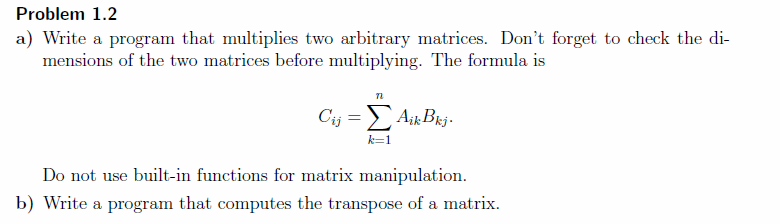
\includegraphics[width=1\textwidth]{chapters/images/desc-1-2}
\end{figure}


\subsubsection{a)}

Multiplying two matrices can be done with the following script:

\begin{lstlisting}[caption=Problem 1.2 a)]
matrix1 = [[1.8, -2], [3, -4.1], [3, 2]];
matrix2 = [[1, -2, -3, 4], [-5, 4, 1, 1]];

print("matrix A:");
mylib.printMatrix(matrix1);

print("matrix B:");
mylib.printMatrix(matrix2);

print("A x B:");

matrix1Rows = len(matrix1);
matrix2Rows = len(matrix2);

matrix1Cols = len(matrix1[0]);
matrix2Cols = len(matrix2[0]);

resultMatrix = [];

if matrix1Cols != matrix2Rows:
	print("number of matrix A columns and matrix B rows aren't equal");

for matrix1Row in range(matrix1Rows):

	resultVector = [];
	for matrix2Col in range(matrix2Cols):
		
		mySum = 0;
		
		for k in range(matrix1Cols):
			mySum = mySum + matrix1[matrix1Row][k] * matrix2[k][matrix2Col];
		
		resultVector.append(mySum);
		
	resultMatrix.append(resultVector);

mylib.printMatrix(resultMatrix);
\end{lstlisting}

The result of the multiplication of the two matrices defined in the script is:

\begin{lstlisting}[caption=Result of 1.2 a), keywordstyle=\color{black}]
matrix A:
    1.8    -2.0
    3.0    -4.1
    3.0     2.0

matrix B:
    1.0    -2.0    -3.0     4.0
   -5.0     4.0     1.0     1.0

A x B:
   11.8   -11.6    -7.4     5.2
   23.5   -22.4   -13.1     7.9
   -7.0     2.0    -7.0    14.0
\end{lstlisting}

\subsubsection{b)}

Transposing a matrix can be done easily with an own function as well:

\begin{lstlisting}[caption=Problem 1.2 b)]
matrix3 = [[1, 2.4], [3.3, -4], [-5, -6.1]];

print("matrix C:");
mylib.printMatrix(matrix3);

matrix3Rows = len(matrix3);
matrix3Cols = len(matrix3[0]);

transposedMatrix = [];

for j in range(matrix3Cols):
	transposedVector = [];

	for i in range(matrix3Rows):
		transposedVector.append(matrix3[i][j]);
	
	transposedMatrix.append(transposedVector);

print("C transposed:");
mylib.printMatrix(transposedMatrix);
\end{lstlisting}

The result is:

\begin{lstlisting}[caption=Result of 1.2 b), keywordstyle=\color{black}]
matrix C:
    1.0     2.4
    3.3    -4.0
   -5.0    -6.1

C transposed:
    1.0     3.3    -5.0
    2.4    -4.0    -6.1
\end{lstlisting}

\section{Calculus - Selected Topics}


\subsection{Problem 2.3}


\begin{figure}[!ht]
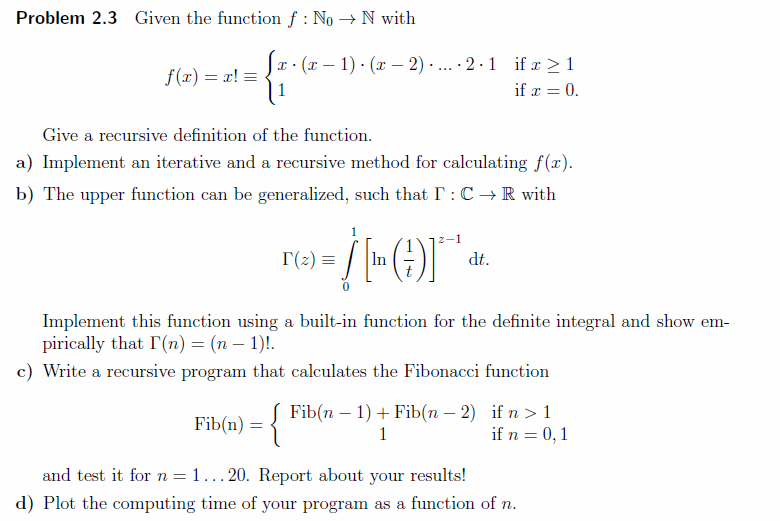
\includegraphics[width=1\textwidth]{chapters/images/desc-2-3}
\end{figure}


\subsubsection{a)}

\begin{lstlisting}[caption=Problem 2.3 a)]
n = int(input("n = "));

factorialIterative = 1;

for i in range(n):
    factorialIterative *= (i + 1);

print("iterative result: " + str(factorialIterative));

def factorialFunc(x):
    if x <= 0: return 1;
	
    return x * factorialFunc(x - 1);

factorialRecursive = factorialFunc(n);

print("recursive result: " + str(factorialRecursive));
\end{lstlisting}

The results of both factorial functions are:

\begin{lstlisting}[caption=Result of 2.3 a), keywordstyle=\color{black}]
n = 9
iterative result: 362880
recursive result: 362880
\end{lstlisting}


\subsubsection{b)}

The integral can be calculated with a built-in function from the scipy library.

\begin{lstlisting}[caption=Problem 2.3 b)]
import scipy.integrate as itg;

def bFunc(t, z):
	return math.pow(math.log(1 / t), z - 1);

for i in range(1, 7):
	factorialResult = factorialFunc(i - 1);
	integrateResult = itg.quad(lambda x: bFunc(x, i), 0, 1);
	
	print("n = " + str(i));
	print("(n - 1)! = " + str(factorialResult));
	print("Gamma(n) = " + str(integrateResult));
\end{lstlisting}

The results are:

\begin{lstlisting}[caption=Result of 2.3 b), keywordstyle=\color{black}]
n = 1
(n - 1)! = 1
Gamma(n) = (1.0, 1.1102230246251565e-14)

n = 2
(n - 1)! = 1
Gamma(n) = (1.0000000000000004, 1.6653345369377348e-15)

n = 3
(n - 1)! = 2
Gamma(n) = (2.0000000000000018, 1.687538997430238e-14)

n = 4
(n - 1)! = 6
Gamma(n) = (6.000000000000022, 2.9398705692074145e-13)

n = 5
(n - 1)! = 24
Gamma(n) = (24.00000000000007, 3.4425795547576854e-12)

n = 6
(n - 1)! = 120
Gamma(n) = (120.00000000002257, 2.0904167286062147e-10)
\end{lstlisting}

The values of the gamma function are not exact because the quad function only calculates an approximation. The second value that's returned is an estimation of the error.

\subsubsection{c)}

\begin{lstlisting}[caption=Problem 2.3 c)]
def fibonacciFunc(x):
	if x <= 1: return 1;
	
	return fibonacciFunc(x - 1) + fibonacciFunc(x - 2);

for i in range(1, 21):
	fib = fibonacciFunc(i);
	print("fib(" + str(i) + ") = " + str(fib));
\end{lstlisting}

The calculated elements of the Fibonacci sequence are:

\begin{lstlisting}[caption=Result of 2.3 c), keywordstyle=\color{black}]
fib(1) = 1
fib(2) = 2
fib(3) = 3
fib(4) = 5
fib(5) = 8
fib(6) = 13
fib(7) = 21
fib(8) = 34
fib(9) = 55
fib(10) = 89
fib(11) = 144
fib(12) = 233
fib(13) = 377
fib(14) = 610
fib(15) = 987
fib(16) = 1597
fib(17) = 2584
fib(18) = 4181
fib(19) = 6765
fib(20) = 10946
\end{lstlisting}

As it can be seen, the Fibonacci function seems to grow exponentially.


\subsubsection{d)}

\begin{lstlisting}[caption=Problem 2.3 d)]
runtimes = [];

for i in range(30):
	timeStart = time.time();
	fibonacciFunc(i);
	ms = 1000 * (time.time() - timeStart);
	runtimes.append(ms);

plt.plot(runtimes);
plt.xlabel('x');
plt.ylabel('runtime fib(x) [ms]');
plt.show();
\end{lstlisting}

The graph of the runtime of the Fibonacci sequence looks like this:

\begin{figure}[!ht]
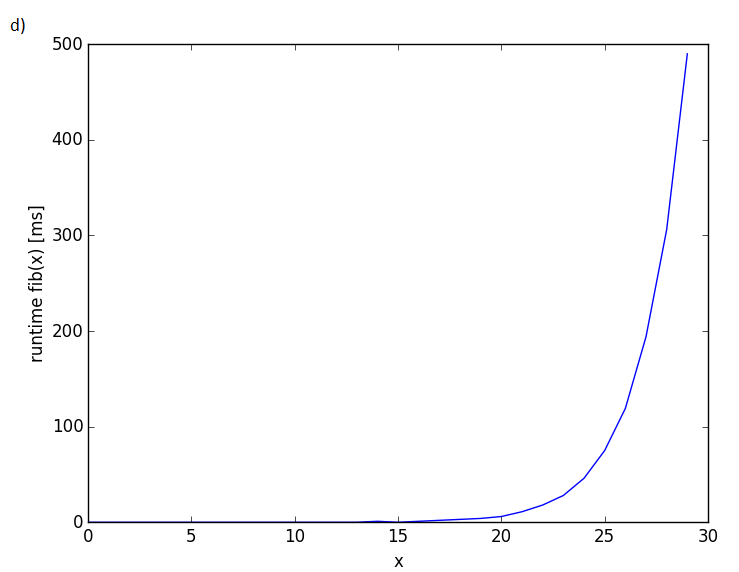
\includegraphics[width=1\textwidth]{chapters/images/figure-2-3-d}
\caption{Runtime of the Fibonacci function}
\end{figure}

As well as the $y$ values of the Fibonacci function, its runtime seems to grow exponentially too.


\subsection{Problem 2.4}

%\begin{figure}[!ht]
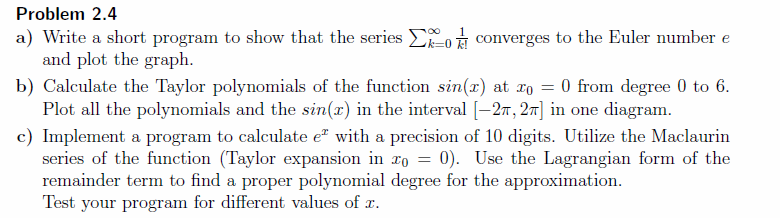
\includegraphics[width=1\textwidth]{chapters/images/desc-2-4}
%\end{figure}


\subsubsection{a)}

To graphically show that the series converges to the Euler number $e$, the series could be defined as a function $f(x)$ where $x$ defines the number of iterations of the sum, like $f(x) = \sum_{k = 0}^{\lfloor x \rfloor} \frac{1}{k!}$.

\begin{lstlisting}[caption=Problem 2.4 a)]
def factorialFunc(x):
    if x <= 0: return 1;
	
    return x * factorialFunc(x - 1);

def aFunc(x):
	sum = 0
	for i in range(x):
		sum += (1.0 / factorialFunc(i));
	return sum;

results = [];
eulers = [];

for i in range(10):
	results.append(aFunc(i));
	eulers.append(math.e);

plt.plot(results);
plt.plot(eulers);
plt.xlabel('x');
plt.ylabel('y');
plt.show();
\end{lstlisting}

The graph of the function with a line for $e$ looks like this:

\newpage

\begin{figure}[!ht]
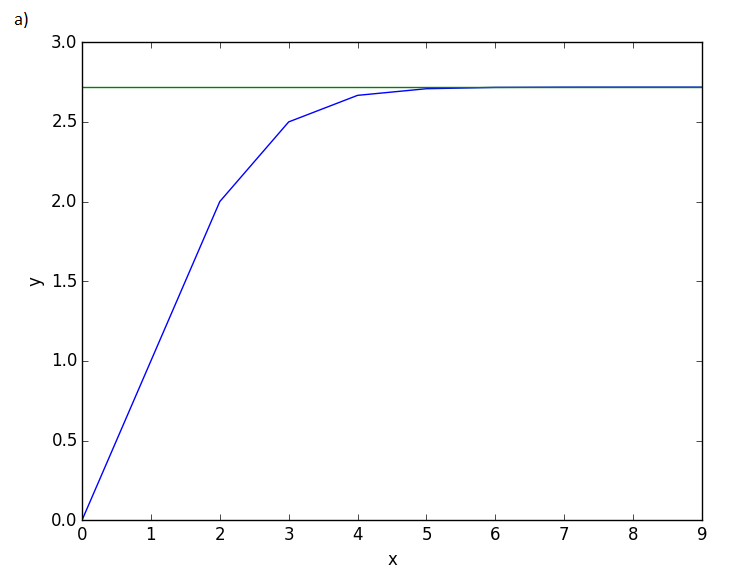
\includegraphics[width=1\textwidth]{chapters/images/figure-2-4-a}
\caption{Graphs of both functions}
\end{figure}

As it can be seen, after $x = 5$ there's hardly any difference visible in the graph.


\subsubsection{b)}

\begin{lstlisting}[caption=Problem 2.4 b)]
def bFunc(degree, x):
	sum = x;
	
	if (degree >= 3): sum -= (1.0 / 6.0) * pow(x, 3);
	if (degree >= 5): sum += (1.0 / 120.0) * pow(x, 5);
	
	return sum;

def bFunc2(degree):
	nSteps = 40;
	xStep = 4 * math.pi / (nSteps - 1);
	x = math.pi * -2;
	
	xses = [];
	results = [];
	
	for i in range(nSteps):
		xses.append(x);
		results.append(bFunc(degree, x));
		x += xStep;
	
	return [xses, results];

for i in range(0, 7):
	taylorFunc = bFunc2(i);
	plt.plot(taylorFunc[0], taylorFunc[1]);

plt.xlabel('x');
plt.ylabel('y');
plt.show();
\end{lstlisting}


The graph of the polynomials looks like the following:

\begin{figure}[!ht]
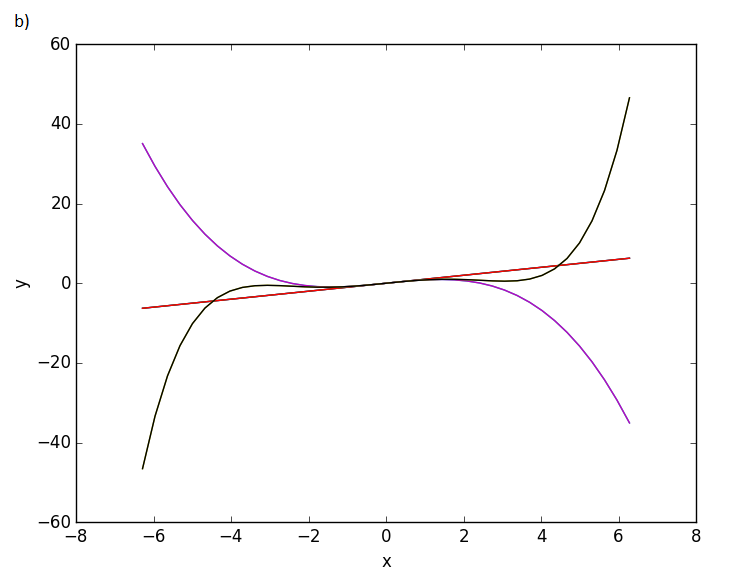
\includegraphics[width=1\textwidth]{chapters/images/figure-2-4-b}
\caption{Graphs of all Taylor series}
\end{figure}

Since $sin^{(2n)}(0) = 0$ for $n \in \mathbb{N}$, the respective term won't show up in the Taylor polynomial. Therefore, the Taylor polynomial for degree $(2n - 1)$ is the same as for degree $(2n)$ (with $n \in \mathbb{N}$). Because of that, only three different polynomials can be seen in the graph.

\subsubsection{c)}

\begin{lstlisting}[caption=Problem 2.4 c)]
ef eulerFunc(d, x):
	if (d <= 0): return 1;

	sum = 1;
	
	for i in range(1, d + 1):
		sum += pow(x, i) / (factorialFunc(i) + 0.0);
	
	return sum;

def getRemainder(n, x):
	xabs = abs(x);
	
	return (math.exp(xabs) * pow(xabs, n + 1)) / float(factorialFunc(n + 1));

def getDegree(x):
	n = 0;
	
	while n < 100:
		remainder = getRemainder(n, x);
		
		if (remainder < 1e-11): return n;
		
		n = n + 1;
		
	return -1;

for x in range(1, 6):
	deg = getDegree(x);
	eul = eulerFunc(deg, x);
	
	print("x = " + str(x) + " | degree = " + str(deg) + " | e(" + str(x) + ") = " + str(eul));
\end{lstlisting}


The resulting approximations as well as the necessary degree for the approximation to be as precise as wanted are the following:

\begin{lstlisting}[caption=Result of 2.4 c), keywordstyle=\color{black}]
x = 1 | degree = 14 | e(1) = 2.71828182846
x = 2 | degree = 19 | e(2) = 7.38905609893
x = 3 | degree = 23 | e(3) = 20.0855369232
x = 4 | degree = 28 | e(4) = 54.5981500331
x = 5 | degree = 32 | e(5) = 148.413159103
\end{lstlisting}

As it can be seen, with every step of $x$ the necessary degree has to increase by about 5.


\subsection{Problem 2.5}

\begin{figure}[!ht]
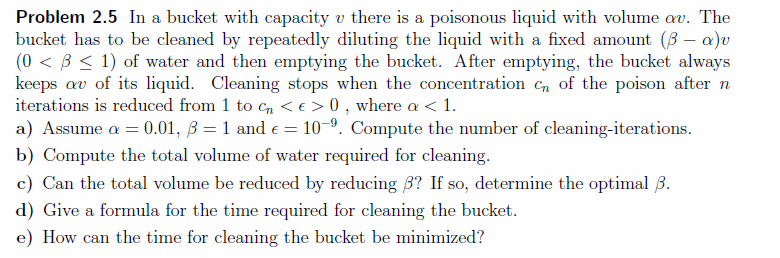
\includegraphics[width=1\textwidth]{chapters/images/desc-2-5}
\end{figure}


\subsubsection{a)}

With each cleaning iteration the concentration is multiplied by $\frac{\alpha}{\alpha + (\beta - \alpha)}$, which can be simplified to $\frac{\alpha}{\beta}$. The bucket can be defined as a class, with $\alpha$, $\beta$ and $\epsilon$ as attributes and the cleaning algorithm as function:

\begin{lstlisting}[caption=Problem 2.5 a)]
class Bucket:
	poison = 1;
	cleaningIterations = 0;
	waterUsed = 0;
	
	def __init__(self, alpha, beta, eps):
		self.alpha = alpha;
		self.beta = beta;
		self.eps = eps;
	
	def doOneClean(self):
		water = self.beta - self.alpha;
		self.waterUsed += water;
		
		self.poison = (self.alpha / float(self.beta)) * self.poison;
	
	def clean(self):
		while (self.poison >= self.eps):
			self.cleaningIterations += 1;
			self.doOneClean();

bu = Bucket(0.01, 1, 10e-9);
bu.clean();
\end{lstlisting}

The result is the following:

\begin{lstlisting}[caption=Result of 2.5 a), keywordstyle=\color{black}]
number of iterations: 5
\end{lstlisting}


\subsubsection{b)}

The necessary adjustments to the class are already in the code fragment of the subtask a) (lines 4 and 13). The result of the calculation is:

\begin{lstlisting}[caption=Result of 2.5 b), keywordstyle=\color{black}]
water used: 4.95 * v
\end{lstlisting}


\subsubsection{c)}

To calculate how much water is needed to reduce the poison to the required concentration, first a formula to calculate the number of required iterations is needed.
The concentration after $n$ iterations is $(\frac{\alpha}{\beta})^n$, which means the number of iterations to reach the required concentration $\epsilon$ is $\lceil log_{\frac{\alpha}{\beta}}(\epsilon) \rceil$.

The amount of water which is used per iteration is $(\beta - \alpha) * v$. Therefore, the amount of water required is $\lceil log_{\frac{\alpha}{\beta}}(\epsilon) \rceil * (\beta - \alpha) * v$.

To find out the optimal $\beta$ with $\alpha = 0.01$ and $\epsilon = 10^{-9}$, the calculation for the water that is needed can be defined as a function $f(\beta) = \lceil log_{\frac{0.01}{\beta}}(10^{-9}) \rceil * (\beta - 0.01)$ with $\beta \in (0, 1]$. Looking at the graph of this function shows that the lowest $y$ value is approaching 0, however the exercise description stated that the water is dilluted with $((\beta - \alpha) * v)$ of water, so the value of $\beta$ has to be greater than $\alpha$. Therefore the optimal $\beta$ in terms of water needed is the lowest possible value that is greater than $\alpha$.


\subsubsection{d)}

As already discovered in the previous subtask, the algorithm to determine the number of iterations is $\lceil log_{\frac{\alpha}{\beta}}(\epsilon) \rceil$. The cleaning time is the result of this calculation times the amount time required for one iteration.

\subsubsection{e)}

The number of iterations, which is proportional to the cleaning time, get smaller the smaller $\frac{\alpha}{\beta}$ is. Therefore, with $\alpha$ as small and $\beta$ as big as possible the time for cleaning the bucket can be minimized. Assuming that $\alpha$ can't be adjusted the best possible value for $\beta$ would be 1.


\section{Statistics and Probability}


\subsection{Problem 3.6}


\begin{figure}[!ht]
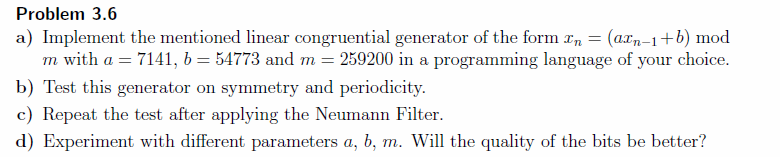
\includegraphics[width=1\textwidth]{chapters/images/desc-3-6}
\end{figure}


\subsubsection{a)}

class for RNG

\begin{lstlisting}[caption=Problem 3.6 a)]
class RNG:
	
	def __init__(self, pA = 7141, pB = 54773, pM = 259200):
		self.bits = [];
		self.x = 1;
		self.a = pA;
		self.b = pB;
		self.m = pM;
	
	def printParameters(self):
		print("a = " + str(self.a) + ", b = " + str(self.b) + ", m = " + str(self.m));
	
	def getRandomNumber(self):
		self.x = (self.a * self.x + self.b) % self.m;
		return self.x;
	
	def addNumbers(self, number):
		binNumber = bin(number)[2:];
		
		for bitNumber in binNumber:
			self.bits.append(int(bitNumber));
	
	def fillNumbers(self, iterations):
		for i in range(iterations):
			self.addNumbers(self.getRandomNumber());
\end{lstlisting}


\subsubsection{b)}

To test for symmetry and periodicity, new functions can be added to the RNG class from a).

\begin{lstlisting}[caption=Problem 3.6 b)]
	def makeSymmetryTest(self):
		sum = 0;
		
		for b in self.bits:
			sum += b;
		
		deviation = abs(0.5 - (sum / float(len(self.bits))));
		
		print("symmetry test:")
		print("deviation = " + str(deviation));
	
	def isPeriod(self, periodLength):
		nBits = len(self.bits);
		
		if periodLength * 2 > nBits: return False;
		
		iterations = int(math.floor(nBits / float(periodLength)));
		
		for i in range(periodLength):
			compareElement = self.bits[i];
		
			for j in range(1, iterations):
				key = j * periodLength + i;
				
				if key >= nBits: break;
				
				element = self.bits[key];
				
				if element != compareElement:
					return False;
		
		return True;
	
	def makePeriodicityTest(self):
		periodLength = -1;
		
		maximumPeriod = self.m * int(math.ceil(math.log(self.m, 2)));
		
		for i in range(1, maximumPeriod):
			if self.isPeriod(i):
				periodLength = i;
				break;
		
		print("periodicity test:");
		
		if periodLength < -0.5:
			print("no period found.");
		else:
			print("period length = " + str(periodLength));
\end{lstlisting}

Running these tests with the values $a = 7141$, $b = 54773$ and $m = 2592000$ lead to the following results.


\begin{lstlisting}[caption=Result of 3.6 b), keywordstyle=\color{black}]
symmetry test:
deviation = 0.0266565772348

perodicity test:
no period found.
\end{lstlisting}

Note: The periodicty test had been aborted prematurely due to excessive run times of the program. With the large value $m$ and the conversion of the numbers into binary the length of the period cannot be calculated within reasonable time.


\subsubsection{c)}

Applying the Neumann Filter can also be realized as an additional function for the RNG class:

\begin{lstlisting}[caption=Problem 3.6 c)]
	def applyNeumannFilter(self):
		tempBits = self.bits;
		self.bits = [];
		
		nIterations = int(math.floor(len(tempBits) / 2.0));
		
		for i in range(nIterations):
			bit1 = tempBits[i * 2];
			bit2 = tempBits[i * 2 + 1];
			
			if (bit1 == 0 and bit2 == 1):
				self.bits.append(0);
			elif (bit1 == 1 and bit2 == 0):
				self.bits.append(1);
\end{lstlisting}

The results with the same values of b) after applying the Neumann Filter are:

\begin{lstlisting}[caption=Result of 3.6 c), keywordstyle=\color{black}]
symmetry test:
deviation = 0.000162239945826

perodicity test:
no period found.
\end{lstlisting}

Again, the periodicity test has been aborted prematurely.


\subsubsection{d)}

With the RNG class the values of $a$, $b$ and $m$ can easily be changed for further experiments:

\begin{lstlisting}[caption=Result of 3.6 d), keywordstyle=\color{black}]
a = 1, b = 1, m = 20
symmetry test:
deviation = 0.0769230769231

a = 20, b = 30, m = 100000
symmetry test:
deviation = 0.0624828117265

a = 214013, b = 2531011, m = 4294967296
symmetry test:
deviation = 0.0168803363686
\end{lstlisting}

Looking at the results the deviation tends to get smaller the higher the value of $m$ is. However, even with a value as little as 20 the deviation is somewhat reasonable.

[also a and b prime]


\subsection{Problem 3.7}


\begin{figure}[!ht]
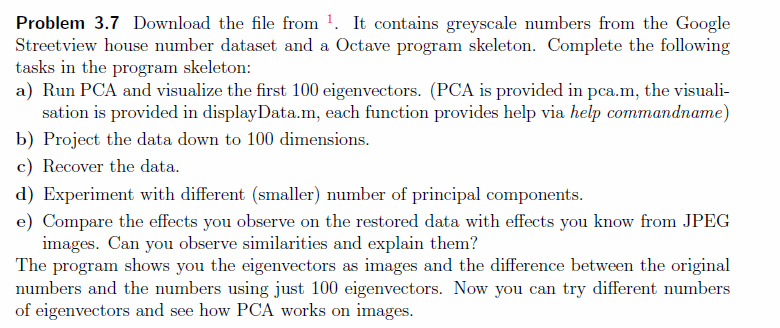
\includegraphics[width=1\textwidth]{chapters/images/desc-3-7}
\end{figure}


\subsubsection{a)}

The first 100 numbers of the data can be dispayed the following way:

\begin{lstlisting}[caption=Problem 3.7 a)]
[U, S] = pca(X_norm);
eigenVectors = U(:,1:100);

displayData(eigenVectors');
\end{lstlisting}

The first 100 numbers of the data looks like this:

\begin{figure}[!ht]
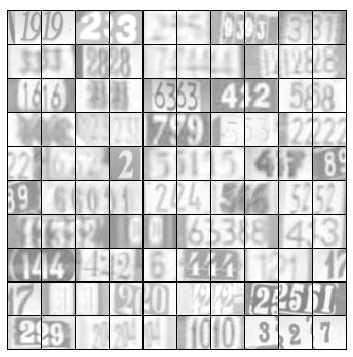
\includegraphics[width=1\textwidth]{chapters/images/figure-3-7-a}
\caption{The first 100 numbers of the data}
\end{figure}

The top 100 eigenvectors

\begin{figure}[!ht]
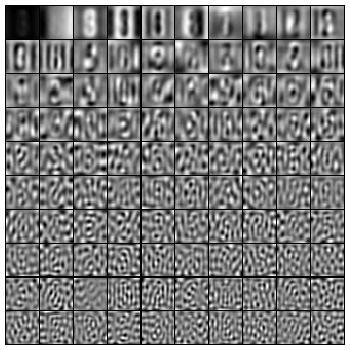
\includegraphics[width=1\textwidth]{chapters/images/figure-3-7-b}
\caption{The top 100 eigenvectors}
\end{figure}

\subsubsection{b)}

To project the data down to 100 dimensions, 

\begin{lstlisting}[caption=Problem 3.7 b)]
Z = X_norm * eigenVectors;
\end{lstlisting}



\subsubsection{c)}

\begin{lstlisting}[caption=Problem 3.7 c)]
recoveredData = Z * eigenVectors';

displayData(X_norm(1:100,:));
displayData(recoveredData(1:100,:));
\end{lstlisting}


results:

\begin{figure}[!ht]
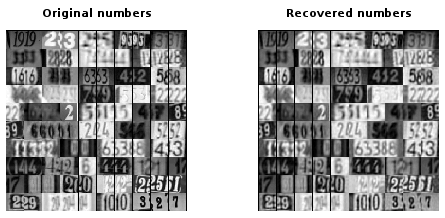
\includegraphics[width=1\textwidth]{chapters/images/figure-3-7-c}
\caption{The data using 100 principal components}
\end{figure}
X



\subsubsection{d)}

\begin{figure}[!ht]
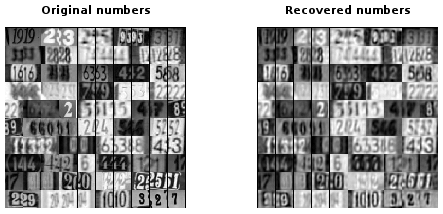
\includegraphics[width=1\textwidth]{chapters/images/figure-3-7-d1}
\caption{The data using 50 principal components}
\end{figure}

\begin{figure}[!ht]
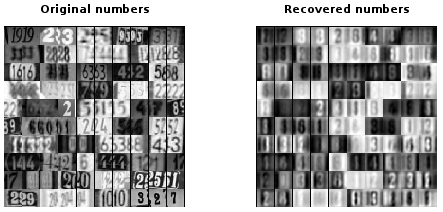
\includegraphics[width=1\textwidth]{chapters/images/figure-3-7-d2}
\caption{The data using 10 principal components}
\end{figure}


\subsubsection{e)}

Like the JPEG compression detail gets lost, especially between two areas where the color contrast is high.

\section{Numerical Mathematics Fundamendals}

\subsection{Problem 4.8}

\begin{figure}[!ht]
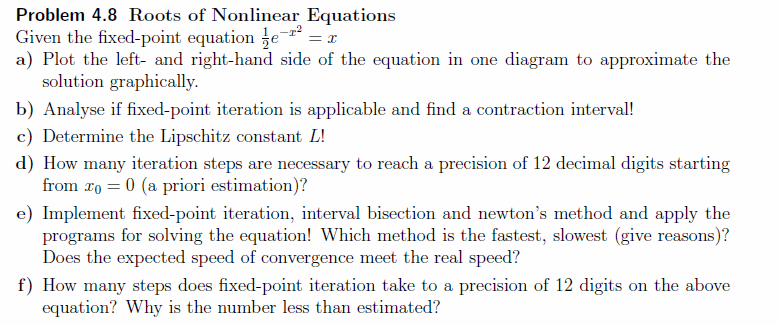
\includegraphics[width=1\textwidth]{chapters/images/desc-4-8}
\end{figure}

First the function needs to be defined. The're are two ways to find a root, setting function equal to $0$ and setting the function equal to $x$. The function which is to be set equal to $0$ is going to be called $f(x)$, while the function to be set equal to $x$ is going to be called $fFixed(x)$, with their derived functions $fDerived(x)$ and $fFixedDerived$ respectively:

\begin{lstlisting}[caption=Different functions for the equation]
def fFixed(x):
	return 0.5 * pow(math.e, -pow(x, 2));

def fFixedDerived(x):
	return -pow(math.e, -pow(x, 2)) * x;

def f(x):
	return fFixed(x) - x;

def fDerived(x):
	return fFixedDerived(x) - 1;
\end{lstlisting}

These functions will be used in the code of the following subtasks, where method to find a root determines which of them is going to be used.


\subsubsection{a)}

With the following code both sides of the equation will be plotted:

\begin{lstlisting}[caption=Problem 4.8 a)]
xses = [];
fLeft = [];
fRight = [];

for i in range(200):
	x = (i / 100.0) - 1;
	
	xses.append(x);
	fLeft.append(fFixed(x));
	fRight.append(x);

plt.plot(xses, fLeft);
plt.plot(xses, fRight);
plt.xlabel('x');
plt.ylabel('y');
plt.show();
\end{lstlisting}

The resulting plot of both sides of the equation looks like the following:

\begin{figure}[!ht]
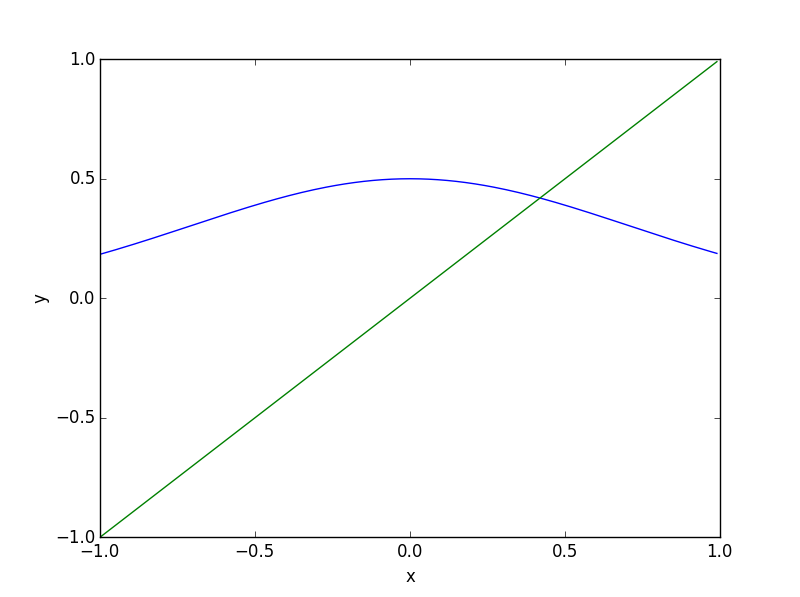
\includegraphics[width=1\textwidth]{chapters/images/figure-4-8-a}
\caption{Graphical solution for the root}
\end{figure}

The approximate solution can be found graphically by looking for an intersection of both functions. The functions intersect close to the point $(0.45~|~0.45)$, therefore the root of the function is approximately 0.45.


\subsubsection{b)}

To use the fixed point interation method for finding a root of a function within an interval $[a, b] \rightarrow [a, b]$, the function has to be a contraction within this interval. A function is a contraction if the Lipschitz constant $L$ is greater than $0$ and smaller than $1$. Within the interval $[0, 1] \rightarrow [0, 1]$, where we graphically estimated the root in the sub task a), the Lipschitz constant is about $0.4289$ (see sub task c)), therefore the condition holds and fixed point interation is applicable.

\subsubsection{c)}

The Lipschitz constant is the highest increase or decrease of a function, or in other words the maximum of the absolute value of the minimum and maximum of the first derivative of said function.
The second derivative of the function has two roots, at $x_1 = -0.70711$ and $x_2 = 0.70711$. These are the maxima and minima of the first derivative, and therefore the highest increase of the function and the Lipschitz constant $L$. Since only $x_2$ is in the contraction interval, the Lipschitz constant can simply be calculated by plugging it into the function $f$.

\begin{lstlisting}[caption=Problem 4.8 c)]
# -0.70711 and 0.70711 are roots of the 2nd derivative of f
lipschitz = abs(fFixedDerived(0.70711));

print("L = " + str(lipschitz));
\end{lstlisting}

The resulting $L$ is:

\begin{lstlisting}[caption=Result of 4.8 c), keywordstyle=\color{black}]
L = 0.428881942471
\end{lstlisting}

\subsubsection{d)}

With the Lipschitz constant from c), the maximum number of iterations required to find a root with a given precision by using the fixed point iteration method can be calculated with the a priori estimation:

\begin{lstlisting}[caption=Problem 4.8 d)]
steps = 0;
err = 1;
xdiff = f(0);

while err > 1e-12:
	steps = steps + 1;
	err = (pow(lipschitz, steps) / (1 - lipschitz)) * xdiff;

print(str(steps) + " iteration steps required");
\end{lstlisting}

The result of this estimation is:

\begin{lstlisting}[caption=Result of 4.8 d), keywordstyle=\color{black}]
33 iteration steps required
\end{lstlisting}

Therefore, to get a precision of 12 decimal digits for our function $f$ a maximum of 33 iterations are needed.

\subsubsection{e)}

First we need a function to see whether our calculated value is precise enough:

\begin{lstlisting}[caption=Determine if an approximation is precise enough]
def isPreciseEnough(val, goal, precision):
	f = pow(10, precision);

	return math.floor(val * f) == math.floor(goal * f);
\end{lstlisting}

The implementation of fixed point iteration could be realized in the following way:

\begin{lstlisting}[caption=Fixed point iteration method]
def getFixedPoint(x0, goal, precision):
	x = x0;
	steps = 1;
	
	while steps < 100:
		x = fFixed(x);
		
		if (isPreciseEnough(x, goal, precision)):
			break;
		
		steps = steps + 1;
	
	return steps;
\end{lstlisting}

The interval bisection method can be implemented like this:

\begin{lstlisting}[caption=Interval Bisection method]
def mySign(x):
	return -1 if x < 0 else 1;

def getRootBisection(pXA, pXB, goal, precision):
	xa = pXA;
	xb = pXB;
	xm = -1;
	steps = 1;
	
	while steps < 100:
		xm = xa + (xb - xa) / 2.0;
		
		if (isPreciseEnough(xm, goal, precision)):
			break;
		
		if mySign(f(xa)) != mySign(f(xm)):
			xb = xm;
		else:
			xa = xm;
		
		steps = steps + 1;
	
	return steps;
\end{lstlisting}

Finally a function to approximate the root of a function with Newton's method could be realized the following way:

\begin{lstlisting}[caption=Newton's method]
def getRootNewton(x0, goal, precision):
	x = x0;
	steps = 1;
	
	while steps < 100:
		fD = fDerived(x);
		
		if abs(fD) < 0.00001: fD = 0.00001;
		
		x = x - float(f(x) / float(fD));
		
		if (isPreciseEnough(x, goal, precision)):
			break;
		
		steps = steps + 1;
	
	return steps;
\end{lstlisting}

Afterwards, the three methods can be compared regarding how much time is needed to find the root of the function with the desired precision.

\begin{lstlisting}[caption=Testing the three methods]
def getTime():
	return time.time();

def printTimeDiff(startTime, endTime):
	averageMS = round((endTime - startTime) / 10.0, 5);
	print("average time taken: " + str(averageMS) + " milliseconds");

def findRoot(type, goal, precision, p1 = 0, p2 = 0):
	startTime = getTime();
	
	steps = 0;
	
	for i in range(10000):
		param1 = p1 + 0.000001 * math.sin(i * 7);
	
		if (type == 0): steps = getFixedPoint(param1, goal, precision);
		elif (type == 1): steps = getRootBisection(param1, p2, goal, precision);
		else: steps = getRootNewton(param1, goal, precision);
	
	print("steps taken: " + str(steps));
	printTimeDiff(startTime, getTime());

def getFixedPointRec2(x, maxSteps, stepsTaken):
	newX = fFixed(x);
	
	if stepsTaken < maxSteps:
		return getFixedPointRec2(newX, maxSteps, stepsTaken + 1);
	else:
		return newX;

def getFixedPointRec1(x0, maxSteps):
	return getFixedPointRec2(x0, maxSteps, 1);

# get a precise enough approximation of the root 
fP33 = getFixedPointRec1(0, 100);

precision = 6;
print("correct digits required: " + str(precision));

print("fixed point iteration:");
findRoot(0, fP33, precision, 0, -1);

print("interval bisection:");
findRoot(1, fP33, precision, 0, 1);

print("newton's method:");
findRoot(2, fP33, precision, 0, -1);

precision = 12;
print("correct digits required: " + str(precision));

print("fixed point iteration:");
findRoot(0, fP33, precision, 0, -1);

print("interval bisection:");
findRoot(1, fP33, precision, 0, 1);

print("newtons method:");
findRoot(2, fP33, precision, 0, -1);

precision = 18;
print("correct digits required: " + str(precision));

print("fixed point iteration:");
findRoot(0, fP33, precision, 0, -1);

print("interval bisection:");
findRoot(1, fP33, precision, 0, 1);

print("newtons method:");
findRoot(2, fP33, precision, 0, -1);
\end{lstlisting}

The results of the tests are the following:

\begin{lstlisting}[caption=Result of 4.8 e), keywordstyle=\color{black}]
correct digits required: 6
fixed point iteration:
steps taken: 14
average time taken: 0.0382 milliseconds

interval bisection:
steps taken: 17
average time taken: 0.0914 milliseconds

newtons method:
steps taken: 4
average time taken: 0.0237 milliseconds

correct digits required: 12
fixed point iteration:
steps taken: 27
average time taken: 0.1185 milliseconds

interval bisection:
steps taken: 40
average time taken: 0.2703 milliseconds

newtons method:
steps taken: 4
average time taken: 0.0321 milliseconds

correct digits required: 18
fixed point iteration:
steps taken: 35
average time taken: 0.1501 milliseconds

interval bisection:
steps taken: 51
average time taken: 0.3547 milliseconds

newtons method:
steps taken: 5
average time taken: 0.0377 milliseconds
\end{lstlisting}

As seen Newton's method is much faster than the other two methods, with up to almost a tenth of computational time. The second fastest method is fixed point iteration, while the interval bisection method is the slowest.

The reason why Newton's method is the fastest is because it also utilizes the first derivative of the function, which is a valuable information to find the root quicker. Interval bisection is the slowest method because it doesn't even use the function value unlike fixed point iteration. Instead, the interval is halved halved with each step, no matter how close one bound is to the root of the function (except when the approximation is already precise enough of course).


\subsubsection{f)}

To get a precise enough approximation of the root, 27 steps were needed instead of the estimated 33 steps in d). The reason it took less iterations is because the a priori estimation always asumes the worst case scenario.


\section{Function Approximation}


\subsection{Problem 5.9}


\begin{figure}[!ht]
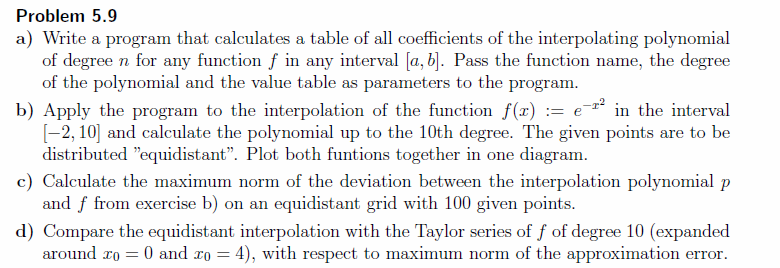
\includegraphics[width=1\textwidth]{chapters/images/desc-5-9}
\end{figure}


\subsubsection{a)}

To calculate the coefficients, [...]

[numpy to solve lin eq]

\begin{lstlisting}[caption=Problem 5.9 a)]
def getCoefficients(fx, degree, a, b):
	xses = [];
	yses = [];
	
	step = (b - a) / float(degree - 1);
	
	for i in range(degree):
		x = a + i * step;
		xses.append(x);
		yses.append(fx(x));
	
	matA = [];
	
	for xVal in xses:
		row = [];
		for i in range(degree):
			row.append(pow(xVal, i));
		
		matA.append(row);
	
	matrixArr = np.array(matA);
	vectorArr = np.array(yses);
	
	linSolutions = np.linalg.solve(matrixArr, vectorArr);
	
	return linSolutions;
\end{lstlisting}

This function will be used in the following subtasks.


\subsubsection{b)}

To use the coefficients as a function, a python function to [return a value is required].

\begin{lstlisting}[caption=Function which uses the calculated coefficients]
def polynomialF(coefficients, x):
	sum = 0.0;
	
	for i in range(len(coefficients)):
		sum += coefficients[i] * pow(x, i);
	
	return sum;
\end{lstlisting}

[now plot them]

\begin{lstlisting}[caption=todo]
def myF(x):
	return pow(math.e, -pow(x, 2));

coefficients = getCoefficients(myF, 10, -2, 10);

xses = [];
realYses = [];
approxYses = [];

for i in range(100):
	x = -2 + i * (12 / 100.0);
	
	xses.append(x);
	realYses.append(myF(x));
	approxYses.append(polynomialF(coefficients, x));

plt.plot(xses, realYses);
plt.plot(xses, approxYses);
plt.xlabel("x");
plt.ylabel("y");
plt.show();
\end{lstlisting}

[the resulting plot looks like the following]

%\begin{figure}[h!]
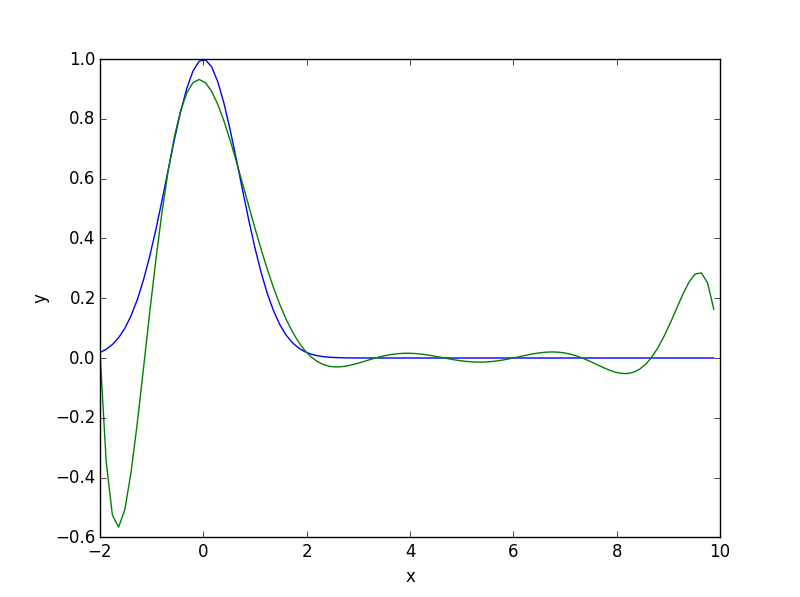
\includegraphics[width=1\textwidth]{chapters/images/figure-5-9-b}
%\caption{Plot of the }
%\end{figure}

\begin{figure}[h!]
%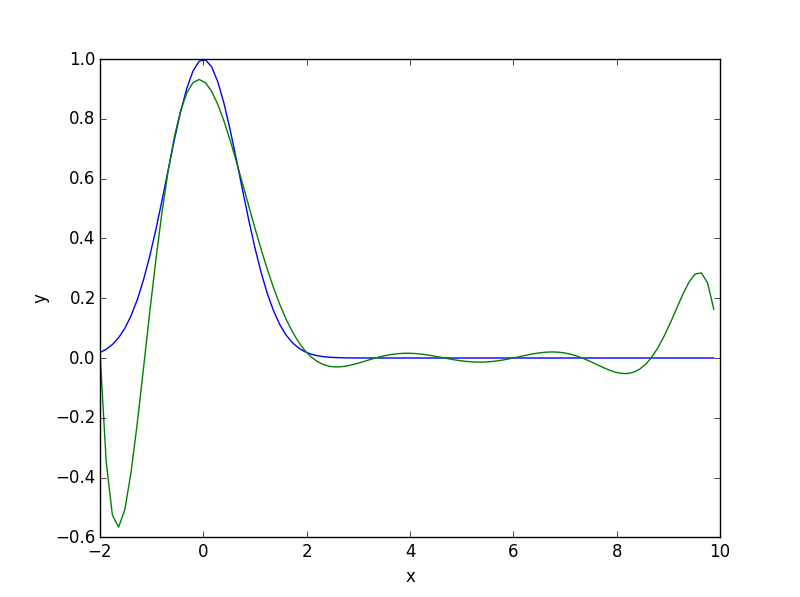
\includegraphics[width=1\textwidth]{chapters/images/figure-5-9-b}
\caption{Plot of both functions}
\end{figure}

[blue - real, green - approx]
[close to origin in the positive part pretty equal]


\subsubsection{c)}

\begin{lstlisting}[caption=Problem 5.9 c)]
maxApproxDev = -1;

for i in range(100):
	realY = realYses[i];
	approxY = approxYses[i];
	
	maxApproxDev = max(maxApproxDev, abs(realY - approxY));

print("maximum deviation: " + str(maxApproxDev));
\end{lstlisting}


The results of the calculation of the maximum deviation are:

\begin{lstlisting}[caption=Result of 5.9 c), keywordstyle=\color{black}]
maximum deviation: 0.634025332357
\end{lstlisting}


\subsubsection{d)}

[First Taylor Series]

[Calc Yses for Plot]

\begin{lstlisting}[caption=todo]
def taylorFuncAt0(x):
	sum = 1;
	sum -= pow(x, 2);
	sum += pow(x, 4) / 2.0;
	sum -= pow(x, 6) / 6.0;
	sum += pow(x, 8) / 24.0;
	sum -= pow(x, 10) / 120.0;
	sum += pow(x, 12) / 720.0;
	sum -= pow(x, 14) / 5040.0;
	sum += pow(x, 16) / 40320.0;
	
	return sum;

def taylorFuncAt4(x):
	ep16 = float(pow(math.e, 16));
	xm4 = x - 4;
	
	sum = 1 / ep16;
	sum -= 8 * xm4 / ep16;
	sum += 31 * pow(xm4, 2) / ep16;
	sum -= 232 * pow(xm4, 3) / (3 * ep16);
	sum += 835 * pow(xm4, 4) / (6 * ep16);
	sum -= 2876 * pow(xm4, 5) / (15 * ep16);
	sum += 18833 * pow(xm4, 6) / (90 * ep16);
	sum -= 58076 * pow(xm4, 7) / (315 * ep16);
	sum += 332777 * pow(xm4, 8) / (2520 * ep16);
	sum -= 43325 * pow(xm4, 9) / (567 * ep16);
	sum += 3937007 * pow(xm4, 10) / (113400 * ep16);
	
	return sum;

taylor0Yses = [];
taylor4Yses = [];

for i in range(100):
	x = -2 + i * (12 / 100.0);
	
	taylor0Yses.append(taylorFuncAt0(x));
	taylor4Yses.append(taylorFuncAt4(x));
\end{lstlisting}

[Then calculate deviation]

\begin{lstlisting}[caption=todo]

maxTaylor0Dev = -1;
maxTaylor4Dev = -1;

for i in range(100):
	realY = realYses[i];
	taylor0Y = taylor0Yses[i];
	taylor4Y = taylor4Yses[i];
	
	maxTaylor0Dev = max(maxTaylor0Dev, abs(realY - taylor0Y));
	maxTaylor4Dev = max(maxTaylor4Dev, abs(realY - taylor4Y));

print("maximum deviation of taylor series with c = 0: " + str(maxTaylor0Dev));
print("maximum deviation of taylor series with c = 4: " + str(maxTaylor4Dev));
\end{lstlisting}

[the results are]

\begin{lstlisting}[caption=Result of 1.1 a), keywordstyle=\color{black}]
maximum deviation of taylor series with c = 0: 1.88827128486e+11
maximum deviation of taylor series with c = 4: 354.936464804
\end{lstlisting}

[taylor at $c = 0$ with much bigger deviation]

[because $c = 4$ is the center of interval]


\subsection{Problem 5.10}


\begin{figure}[!ht]
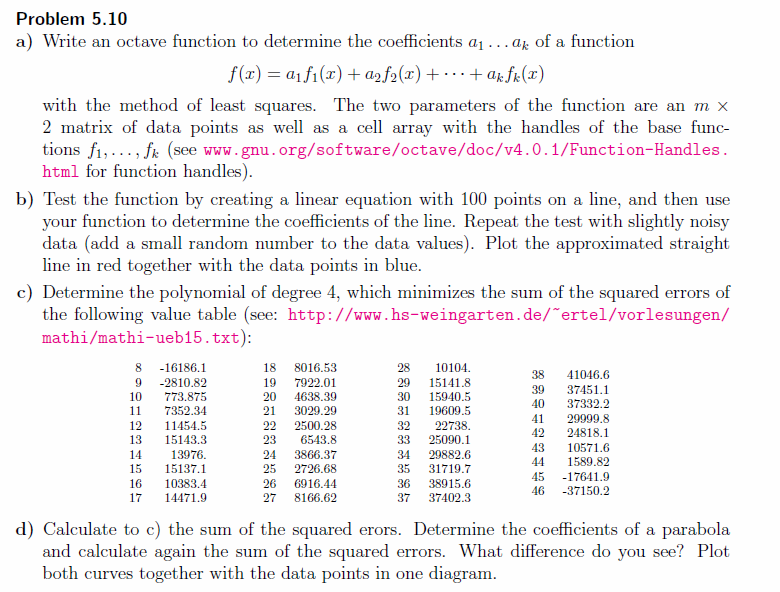
\includegraphics[width=1\textwidth]{chapters/images/desc-5-10}
\end{figure}


\subsubsection{a)}

[get coefficients with method of least squares]

[again lin eq can be solved with numpy]

\begin{lstlisting}[caption=Problem 5.10 a)]
def getCoefficients(baseFunctions, dataPoints):
	l = len(baseFunctions);
	
	matA = [];
	
	for i in range(l):
		matrixRow = [];
		for j in range(l):
			elemSum = 0;
		
			for dp in dataPoints:
				x = dp[0];
				elemSum += baseFunctions[i](x) * baseFunctions[j](x);
			
			matrixRow.append(elemSum);
		
		matA.append(matrixRow);
	
	vecB = [];
	
	for i in range(l):
		elemSum = 0;
	
		for dp in dataPoints:
			elemSum += dp[1] * baseFunctions[i](dp[0]);
		
		vecB.append(elemSum);
	
	matrixArr = np.array(matA);
	vectorArr = np.array(vecB);
	
	linSolutions = np.linalg.solve(matrixArr, vectorArr);
	
	return linSolutions;
\end{lstlisting}


\subsubsection{b)}

[with the function from a), simple to make the lin eq with two base functions.]

[afterwards, calculate enough y values and plot them]

\begin{lstlisting}[caption=todo]
def myF1(x): return x;
def myF0(x): return 1;

baseFns = [];

baseFns.append(myF1);
baseFns.append(myF0);

linPoints = [];
rndPoints = [];
xses = [];
yses = [];
rndYses = [];

for i in range(100):
	x = i / 10.0;
	y = x * 0.64 + 2.3;
	
	xses.append(x);
	yses.append(y);

	rnd = random.random() - 0.5;
	rndY = y + rnd * 0.6;
	rndYses.append(rndY);
	
	linPoints.append([x, y]);
	rndPoints.append([x, rndY]);

print("coefficients:");
print(getCoefficients(baseFns, linPoints));

print("approximated coefficients:");
print(getCoefficients(baseFns, rndPoints));

plt.plot(xses, yses);
plt.plot(xses, rndYses, "ro");
plt.xlabel("x");
plt.ylabel("y");
plt.show();
\end{lstlisting}


[The result of the exact coefficients and the approximation with random points are]

\begin{lstlisting}[caption=Result of 1.1 a), keywordstyle=\color{black}]
coefficients:
[ 0.64   0.23 ]

approximated coefficients:
[ 0.63139257   2.33442881 ]
\end{lstlisting}

[the approximated coefficients are very close.]

[the plot of the exact linear equation and the random points looks like this:]

\begin{figure}[!ht]
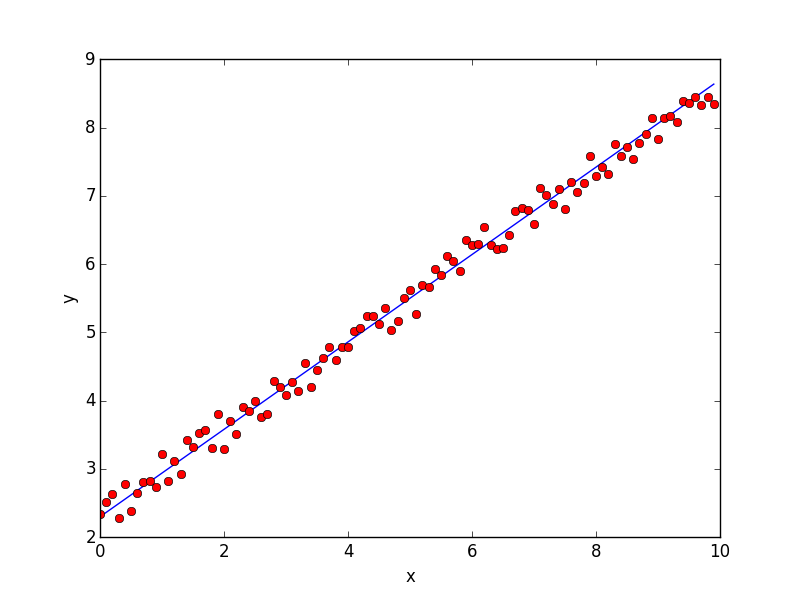
\includegraphics[width=1\textwidth]{chapters/images/figure-5-10-b}
\caption{todo}
\end{figure}


\subsubsection{c)}

[also with the function, poly degree 4 and 2 which is needed for subtask d)]

\begin{lstlisting}[caption=todo]
def myF4(x): return pow(x, 4);
def myF3(x): return pow(x, 3);
def myF2(x): return pow(x, 2);
def myF1(x): return x;
def myF0(x): return 1;

def polynomialF(coefficients, x):
	sum = 0.0;
	
	nc = len(coefficients);
	
	for i in range(nc):
		sum += coefficients[i] * pow(x, nc - i - 1);
	
	return sum;

txtBaseFns4 = [];
txtBaseFns2 = [];

txtBaseFns4.append(myF4);
txtBaseFns4.append(myF3);
txtBaseFns4.append(myF2);
txtBaseFns4.append(myF1);
txtBaseFns4.append(myF0);

txtBaseFns2.append(myF2);
txtBaseFns2.append(myF1);
txtBaseFns2.append(myF0);

txtPoints = [];

txtPoints.append([8, -16186.1]);
txtPoints.append([9, -2810.82]);
# [...] (I left out the other values in the paper to save space)
txtPoints.append([45, -17641.9]);
txtPoints.append([46, -37150.2]);

txtCoefficients4 = getCoefficients(txtBaseFns4, txtPoints);
txtCoefficients2 = getCoefficients(txtBaseFns2, txtPoints);

txtPointsXses = [];
txtPointsYses = [];

error4 = 0;
error2 = 0;

for i in range(len(txtPoints)):
	txtPoint = txtPoints[i];
	
	txtPointsXses.append(txtPoint[0]);
	txtPointsYses.append(txtPoint[1]);
	
	y4 = polynomialF(txtCoefficients4, i + 8);
	y2 = polynomialF(txtCoefficients2, i + 8);
	
	error4 += pow(y4 - txtPoint[1], 2);
	error2 += pow(y2 - txtPoint[1], 2);


print("error of degree 4 polynomial: " + str(error4));
print("error of degree 2 polynomial: " + str(error2));

txtFXses = [];
txtF4Yses = [];
txtF2Yses = [];

for i in range(152):
	x = 8 + i * 0.25;
	
	txtFXses.append(x);
	
	y4 = polynomialF(txtCoefficients4, x);
	y2 = polynomialF(txtCoefficients2, x);
	
	txtF4Yses.append(y4);
	txtF2Yses.append(y2);


plt.plot(txtFXses, txtF4Yses);
plt.plot(txtFXses, txtF2Yses);
plt.plot(txtPointsXses, txtPointsYses, "ro");
plt.xlabel("x");
plt.ylabel("y");
plt.show();
\end{lstlisting}


results:

\begin{lstlisting}[caption=Result of 1.1 a), keywordstyle=\color{black}]
R
\end{lstlisting}

X



\subsubsection{d)}

[use the functions from c) 

\begin{lstlisting}[caption=todo]

siehe c) - aufdroeseln

\end{lstlisting}


results:

\begin{lstlisting}[caption=Result of 1.1 a), keywordstyle=\color{black}]
error of degree 4 polynomial: 101457690.277
error of degree 2 polynomial: 7711489909.2
\end{lstlisting}

[error of degree 4 over 70 times smaller] [makes sense]

[the plot looks like this]

\begin{figure}[!ht]
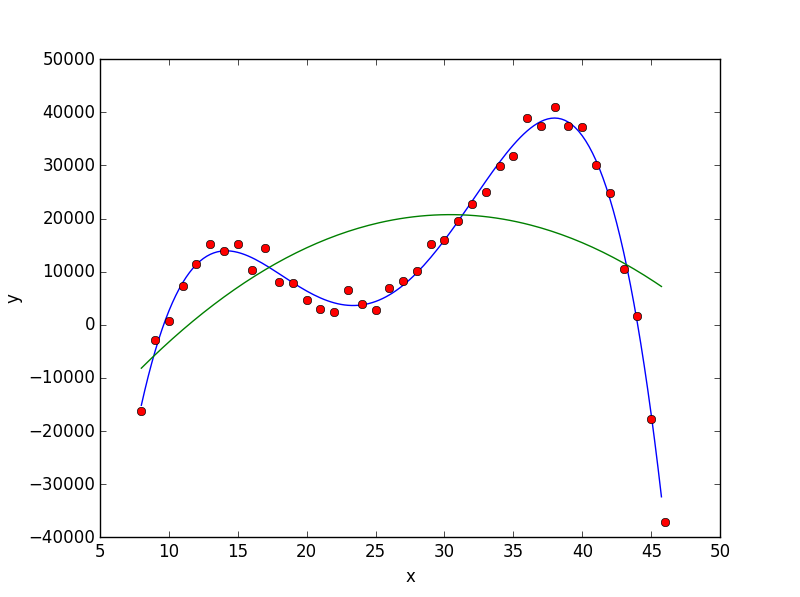
\includegraphics[width=1\textwidth]{chapters/images/figure-5-10-d}
\caption{todo}
\end{figure}

[perfectly illustrates the closeness and farawayness of each function]


\subsection{Problem 5.11}


\begin{figure}[!ht]
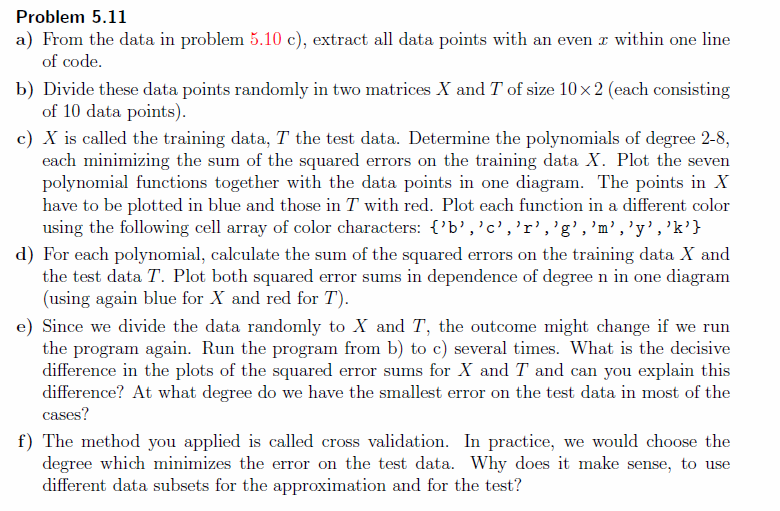
\includegraphics[width=1\textwidth]{chapters/images/desc-5-11}
\end{figure}

The methods $getCoefficients$ and $polynomialF$ as well as the $txtPoints$ from problem 5.10 will be used in this exercise as well.


\subsubsection{a)}

\begin{lstlisting}[caption=todo]
evenPoints = [];

for txtPoint in txtPoints:
	if txtPoint[0] % 2 == 0:
		evenPoints.append(txtPoint);
\end{lstlisting}


\subsubsection{b)}

\begin{lstlisting}[caption=todo]
matrixX = [];
matrixT = [];

for evenPoint in evenPoints:
	rnd = random.random();
	
	if len(matrixT) >= 10 or (rnd < 0.5 and len(matrixX) < 10):
		matrixX.append(evenPoint);
	else:
		matrixT.append(evenPoint);
\end{lstlisting}


\subsubsection{c)}

[To get the polynomials up to degree 8, first the base functions have to be defined:]

\begin{lstlisting}[caption=todo]
def myF8(x): return pow(x, 8);
def myF7(x): return pow(x, 7);
def myF6(x): return pow(x, 6);
def myF5(x): return pow(x, 5);
def myF4(x): return pow(x, 4);
def myF3(x): return pow(x, 3);
def myF2(x): return pow(x, 2);
def myF1(x): return x;
def myF0(x): return 1;

def getBaseFunctionList(degree):
	baseFunctions = [];
	
	if degree >= 8: baseFunctions.append(myF8);
	if degree >= 7: baseFunctions.append(myF7);
	if degree >= 6: baseFunctions.append(myF6);
	if degree >= 5: baseFunctions.append(myF5);
	if degree >= 4: baseFunctions.append(myF4);
	if degree >= 3: baseFunctions.append(myF3);
	if degree >= 2: baseFunctions.append(myF2);
	
	baseFunctions.append(myF1);
	baseFunctions.append(myF0);
	
	return baseFunctions;
\end{lstlisting}

[using these base functions the coefficients can be calculated with the $getCoefficients$ function. Afterwards, the y values of those functions can be collected with the $polynomialF$ function to plot them].

\begin{lstlisting}[caption=todo]
xses = [];
allYses = [];

for i in range(152):
	xses.append(8 + i * 0.25);

for i in range(7):
	degree = i + 2;
	
	baseFunctionList = getBaseFunctionList(degree);
	
	coefficients = getCoefficients(baseFunctionList, matrixX);
	
	yses = [];
	
	for x in xses:
		y = polynomialF(coefficients, x);
		yses.append(y);
	
	allYses.append(yses);

xXses = [];
xYses = [];
tXses = [];
tYses = [];

for i in range(10):
	xXses.append(matrixX[i][0]);
	xYses.append(matrixX[i][1]);
	tXses.append(matrixT[i][0]);
	tYses.append(matrixT[i][1]);

colors = ["b", "c", "r", "g", "m", "y", "k"];

plt.plot(xXses, xYses, "bo");
plt.plot(tXses, tYses, "ro");

for i in range(len(allYses)):
	plt.plot(xses, allYses[i], colors[i]);

plt.xlabel("x");
plt.ylabel("y");
plt.show();
\end{lstlisting}

[the resulting graph looks like this.]

\begin{figure}[!ht]
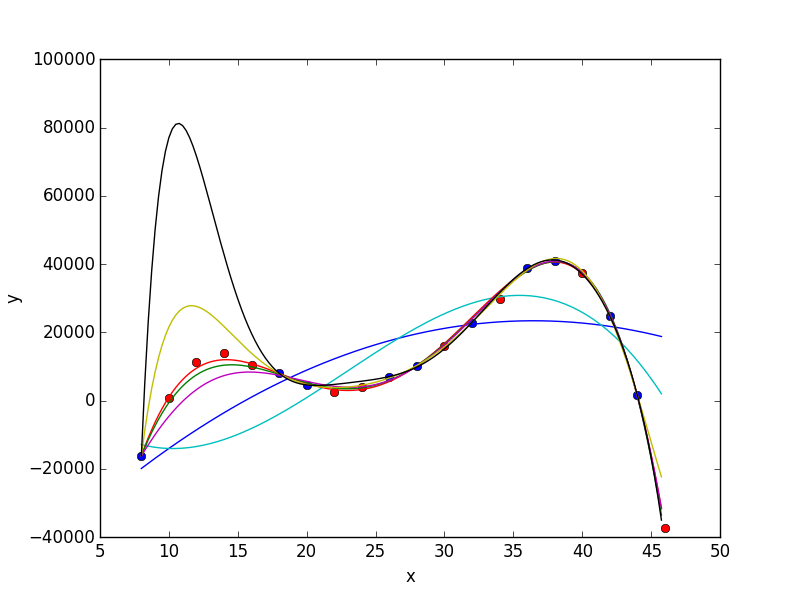
\includegraphics[width=1\textwidth]{chapters/images/figure-5-11-c}
\caption{todo}
\end{figure}


\subsubsection{d)}

[to calculate the error, square of distance between data point]

\begin{lstlisting}[caption=todo]
def getError(coefficients, mat):
	errorSum = 0;
	
	for elem in mat:
		fY = polynomialF(coefficients, elem[0]);
		
		errorSum += pow(fY - elem[1], 2);
	
	return errorSum;

def getErrors(degree, matX, matT):
	baseFunctionList = getBaseFunctionList(degree);
	
	coefficients = getCoefficients(baseFunctionList, matX);
	
	errorSumX = getError(coefficients, matX);
	errorSumT = getError(coefficients, matT);
	
	return [errorSumX, errorSumT];

degrees = [];
errorsX = [];
errorsT = [];

for i in range(7):
	degree = i + 2;
	degrees.append(degree);
	
	errors = getErrors(degree, matrixX, matrixT);
	
	errorsX.append(errors[0]);
	errorsT.append(errors[1]);

plt.plot(degrees, errorsX, "b");
plt.plot(degrees, errorsT, "r");

plt.xlabel("degree");
plt.ylabel("error");
plt.show();
\end{lstlisting}

[the result looks the following:]

\begin{figure}[!ht]
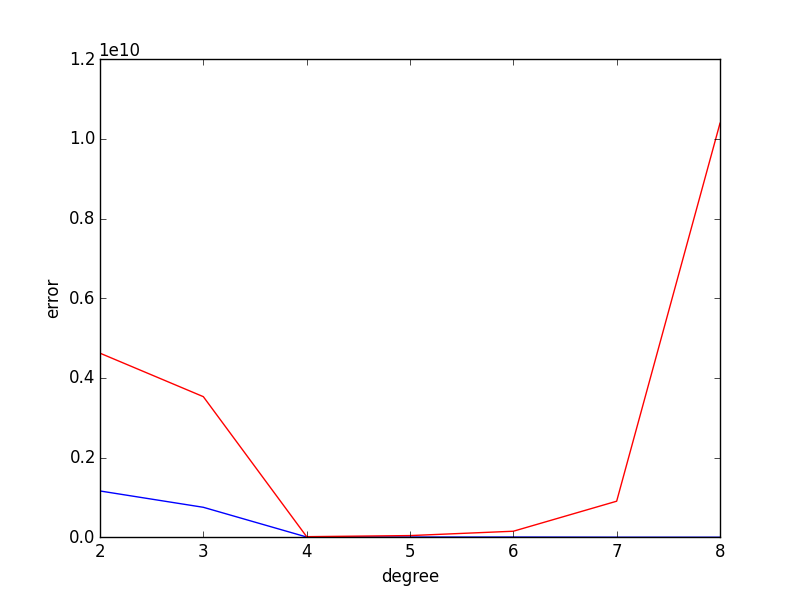
\includegraphics[width=1\textwidth]{chapters/images/figure-5-11-d}
\caption{todo}
\end{figure}


\subsubsection{e)}

[with a higher degree, the deviation from training data is pretty small]. [obv since they are used for the small function]

[on the test data however the error first drops but then increases]

The deviation to the original approximated function (where all data points were used) minimizes the more evenly the points of X and T are distributed. The reason for that is that when there's a large interval of test points only, the approximated function has no bounds at all in that interval and can deviate as much as it needs to, without increasing the error.
The results seems to be the the best with polynomials of degree 4 and 5.

[a reason could be that functions of higher degrees tend to spike more, and they are more free with \enquote{loose} test data points]

\subsubsection{f)}

It makes sense because the approximated function is supposed to be close to all data values, and even the points \enquote{in between} which are not part of both the training and test data.
\section{Numerical Integration and Solution of Ordinatry Diffential Equations}


\subsection{Problem 7.12}


\begin{figure}[!ht]
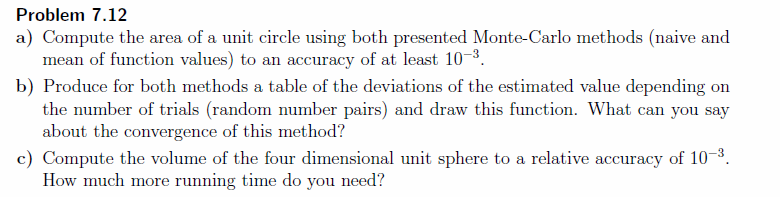
\includegraphics[width=1\textwidth]{chapters/images/desc-7-12}
\end{figure}


\subsubsection{a)}

First we need a function whose integral over a certain interval is equal the area of the unit circle. The integral of the function $\sqrt{1 - x^2}$ over the interval $[-1, 1]$ equals half the area of the unit circle, so with a little tweaking of the parameter $x$ we can modify the function to have an integral equal to the unit circle over the interval $[0, 4]$. The function in Python looks the following way:

\begin{lstlisting}[caption=Function for the unit circle area]
def circleF(x):
	newX = (x % 2) - 1;
	return math.sqrt(1 - pow(newX, 2));
\end{lstlisting}

Afterwards, we can use this function for the calculation of the area with both the naive and mean Monte Carlo method:

\begin{lstlisting}[caption=Problem 7.12 a)]
goal = math.pi;

def getRandCoord(a, b):
	return random.random() * (b - a) + a;

def doNaiveMonteCarloTest(xMin, xMax, yMin, yMax):
	randX = getRandCoord(xMin, xMax);
	randY = getRandCoord(yMin, yMax);
	
	return circleF(randX) > randY;

def doNaiveMonteCarlo(precision):
	areaEstimated = 0;
	tries = 0.0;
	successes = 0.0;

	while abs(areaEstimated - goal) > precision:
		if doNaiveMonteCarloTest(0, 4, 0, 1):
			successes += 1;
		
		tries += 1;
		
		areaEstimated = 4 * (successes / tries);
	
	return [areaEstimated, tries];

def doMeanMonteCarlo(precision):
	areaEstimated = 0;
	tries = 0.0;
	sum = 0.0;
	
	while abs(areaEstimated - goal) > precision:
		randX = getRandCoord(0, 4);
		
		sum += circleF(randX);
		tries += 1;
		
		areaEstimated = 4 * (sum / tries);
	
	return [areaEstimated, tries];

minError = 0.001;

naiveMonteCarlo = doNaiveMonteCarlo(minError);
print("naive method:");
print("estimated area: " + str(naiveMonteCarlo[0]));
print("tries: " + str(naiveMonteCarlo[1]));

meanMonteCarlo = doMeanMonteCarlo(minError);
print("mean value method:");
print("estimated area: " + str(meanMonteCarlo[0]));
print("tries: " + str(meanMonteCarlo[1]));
\end{lstlisting}

The results of those calculations are:

\begin{lstlisting}[caption=Result of 7.12 a), keywordstyle=\color{black}]
naive method:
estimated area: 3.14241702843
tries: 7141.0

mean value method:
estimated area: 3.14239623321
tries: 658.0
\end{lstlisting}


\subsubsection{b)}

To calculate the deviation we can use a slightly alternative version of the Monte Carlo functions of a).

\begin{lstlisting}[caption=Problem 7.13 b)]
def getNaiveMonteCarloDeviation(tries):
	successes = 0.0;
	
	for i in range(tries):
		if doNaiveMonteCarloTest(0, 4, 0, 1):
			successes += 1;
	
	areaEstimated = 4 * (successes / tries);
	
	return abs(areaEstimated - goal);

def getMeanMonteCarloDeviation(tries):
	sum = 0.0;
	
	for i in range(tries):
		randX = getRandCoord(0, 4);
		
		sum += circleF(randX);
	
	areaEstimated = 4 * (sum / tries);
	
	return abs(areaEstimated - goal);

xses = [];
naiveYses = [];
meanYses = [];

for i in range(1, 250):
	naiveDeviation = getNaiveMonteCarloDeviation(i * 10);
	meanDeviation = getMeanMonteCarloDeviation(i * 10);
	
	xses.append(i);
	naiveYses.append(naiveDeviation);
	meanYses.append(meanDeviation);

plt.plot(xses, naiveYses);
plt.plot(xses, meanYses);
plt.xlabel("tries");
plt.ylabel("deviation");
plt.show();
\end{lstlisting}

\newpage

The resulting graph looks like this:

\begin{figure}[!ht]
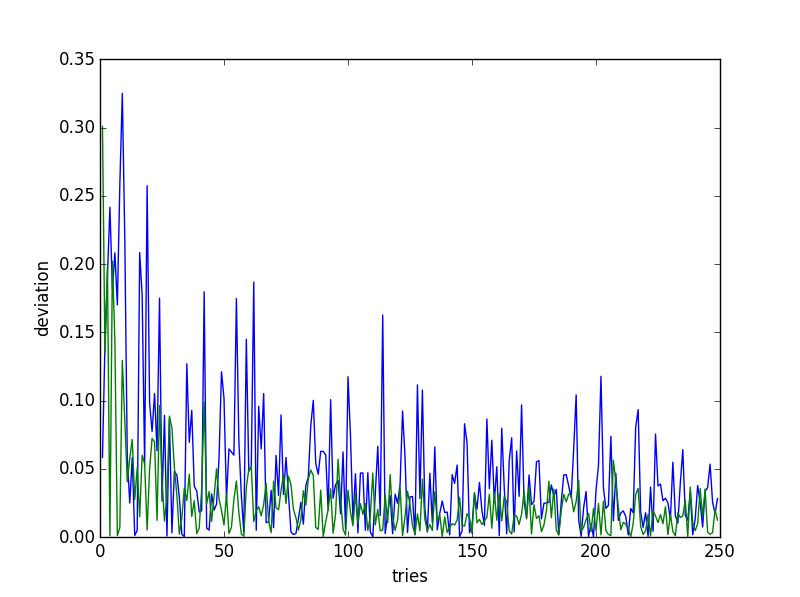
\includegraphics[width=1\textwidth]{chapters/images/figure-7-12-b}
\caption{Deviation of the Monte Carlo methods}
\end{figure}

Although the deviation tends to get smaller and smaller there is no convergence. Due to the random factor both functions have there is no guarantee the $y$ values get close to a certain value.


\subsubsection{c)}

To calculate the volume we again need a function to check whether a random point is within our body of choice. For an n-dimensional unit sphere we can simply check whether the length of the n-dimensional vector of the coordinates is shorter than 1. If so, the point is within the sphere. The Python function for the four-dimensional sphere can be implemented in the following way:

\begin{lstlisting}[caption=Function for the 4D unit sphere volume]
def isIn4DSphere4D(x, y, z, a):
	return math.sqrt(pow(x, 2) + pow(y, 2) + pow(z, 2) + pow(a, 2)) < 1;
\end{lstlisting}

Again we use this function for the Monte Carlo method to calculate the volume the same way we did in the subtask a):

\begin{lstlisting}[caption=4D unit sphere volume calculation]
def doNaiveMonteCarloTest4D():
	randX = getRandCoord(0, 1);
	randY = getRandCoord(0, 1);
	randZ = getRandCoord(0, 1);
	randA = getRandCoord(0, 1);
	
	return isIn4DSphere4D(randX, randY, randZ, randA);

goal2 = pow(math.pi, 2) / 2.0;

def doNaiveMonteCarlo4D(precision):
	areaEstimated = 0;
	tries = 0.0;
	successes = 0.0;

	while abs(areaEstimated - goal2) > precision:
		if doNaiveMonteCarloTest4D():
			successes += 1;
		
		tries += 1;
		
		areaEstimated = 16 * (successes / tries);
	
	return [areaEstimated, tries];

fourDSphere = doNaiveMonteCarlo4D(minError);
print("estimated area of 4D unit sphere: " + str(fourDSphere[0]));
\end{lstlisting}

The result of the calculation is the following:

\begin{lstlisting}[caption=Result of the 4D unit sphere volume calculation, keywordstyle=\color{black}]
estimated area of 4D unit sphere: 4.93493975904
\end{lstlisting}

Afterwards we can analyze the computational time of both methods:

\begin{lstlisting}[caption=Problem 7.12 c)]
total2DTries = 0.0;
total4DTries = 0.0;

runs = 250;

for i in range(runs):
	total2DTries += doNaiveMonteCarlo(minError)[1];
	total4DTries += doNaiveMonteCarlo4D(minError)[1];

avg2DTries = total2DTries / float(runs);
avg4DTries = total4DTries / float(runs);

print("average tries for 2d unit circle: " + str(avg2DTries));
print("average tries for 4d unit sphere: " + str(avg4DTries));
\end{lstlisting}

The results of these calculations are:

\begin{lstlisting}[caption=Result of 7.12 c), keywordstyle=\color{black}]
average tries for 2d unit circle: 4928.92
average tries for 4d unit sphere: 14141.112
\end{lstlisting}

Looking at the results, it takes about 3 times as much computational time to calculate the volume of a 4 dimensional unit sphere than it is to calculate the area of a 2 dimensional unit circle.


\subsection{Problem 7.13}


\begin{figure}[!ht]
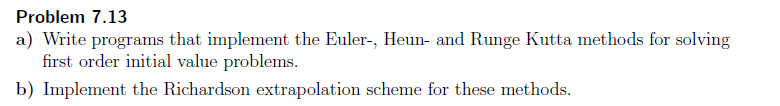
\includegraphics[width=1\textwidth]{chapters/images/desc-7-13}
\end{figure}


\subsubsection{a)}

To solve an ODE, first a general function can be defined for the basic approach. To make this function applicable for different approximation methods (like Euler method and Runge-Kutta method) the function which defines how to calculate the $y_{n + 1}$ value will be passed as an argument. This abstract function will be called \textit{yp1Method} in this exercise.

\begin{lstlisting}[caption=Function to solve ODE]
def odeSolver(f, a, b, y0, h, yp1Method):
	x = a;
	y = y0;
	
	yses = [];
	yses.append(y);
	
	while x <= b:
		y = yp1Method(f, x, y, h);
		yses.append(y);
		
		x += h;
	
	return yses;
\end{lstlisting}

Afterwards, we need to define the \textit{yp1Method} functions for the Euler, Heun, and Runge-Kutta methods.

\begin{lstlisting}[caption=YP1Methods]
def eulerYP1(f, x, y, h):
	return y + h * f(x, y);

def heunYP1(f, x, y, h):
	k1 = h * f(x, y);
	k2 = h * f(x + h, y + k1);
	
	return y + 0.5 * (k1 + k2);

def rungeKuttaYP1(f, x, y, h):
	k1 = h * f(x, y);
	k2 = h * f(x + 0.5 * h, y + 0.5 * k1);
	k3 = h * f(x + 0.5 * h, y + 0.5 * k2);
	k4 = h * f(x + h, y + k3);
	
	return y + (1 / 6.0) * (k1 + 2 * k2 + 2 * k3 + k4);
\end{lstlisting}

The final ODE solving functions for each method can now call the basic \textit{odeSolver} function and pass the respective \textit{yp1Method}:

\begin{lstlisting}[caption=ODE solving functions for each method]
def euler(f, a, b, y0, h):
	return odeSolver(f, a, b, y0, h, eulerYP1);

def heun(f, a, b, y0, h):
	return odeSolver(f, a, b, y0, h, heunYP1);

def rungeKutta(f, a, b, y0, h):
	return odeSolver(f, a, b, y0, h, rungeKuttaYP1);
\end{lstlisting}

To solve an ODE system the function has to be altered a little bit.

\begin{lstlisting}[caption=Function to solve an ODE system]
def odeSystemSolver(fVector, a, b, y0Vector, h, yp1Methods):
	yVectorses = [];
	
	x = a;
	yVector = y0Vector;
	
	yVectorses.append(yVector);
	
	while x <= b:
		yp1Vector = yp1Methods(fVector, x, yVector, h);
		
		yVectorses.append(yp1Vector);
		
		yVector = yp1Vector;
		
		x += h;
	
	return yVectorses;
\end{lstlisting}

Also a new \textit{yp1Method} has to be defined:

\begin{lstlisting}[caption=YP1Method for solving an ODE system]
def rungeKuttaYP1System(fVector, x, yVector, h):
	nF = len(fVector);
	
	k1Vector = [];
	yVectorPlusHalfK1Vector = [];
	
	for i in range(nF):
		k1El = h * fVector[i](x, yVector);
		k1Vector.append(k1El);
		yVectorPlusHalfK1Vector.append(yVector[i] + 0.5 * k1El);
	
	k2Vector = [];
	yVectorPlusHalfK2Vector = [];
	
	for i in range(nF):
		k2El = h * fVector[i](x + 0.5 * h, yVectorPlusHalfK1Vector);
		k2Vector.append(k2El);
		yVectorPlusHalfK2Vector.append(yVector[i] + 0.5 * k2El);
	
	k3Vector = [];
	yVectorPlusK3Vector = [];
	
	for i in range(nF):
		k3El = h * fVector[i](x + 0.5 * h, yVectorPlusHalfK2Vector);
		k3Vector.append(k3El);
		yVectorPlusK3Vector.append(yVector[i] + k3El);
	
	yp1Vector = [];
	
	for i in range(nF):
		k4El = h * fVector[i](x + h, yVectorPlusK3Vector);
		
		yp1 = yVector[i] + (1 / 6.0) * (k1Vector[i] + 2 * k2Vector[i] + 2 * k3Vector[i] + k4El);
		
		yp1Vector.append(yp1);
	
	return yp1Vector;

def rungeKuttaSystem(fVector, a, b, y0Vector, h):
	return odeSystemSolver(fVector, a, b, y0Vector, h, rungeKuttaYP1System);
\end{lstlisting}


\subsubsection{b)}

For the Richardson extrapolation we need to define new functions for the different \textit{yp1Methods} again to calculate the value of the next $y$ value. However, the basic ODE solving function can be reused.

\begin{lstlisting}[caption=Problem 7.13 b)]
def fkFunc(f, x, y, h, yp1Func, q, pk, step):
	if step == 1:
		fh = yp1Func(f, x, y, h);
		fqh = yp1Func(f, x, y, q * h);
	else:
		fh = fkFunc(f, x, y, h, yp1Func, q, pk, step - 1);
		fqh = fkFunc(f, x, y, q * h, yp1Func, q, pk, step - 1);
	
	return fh + ((fh - fqh) / (pow(q, pk) - 1.0));

def eulerYP1Richardson(f, x, y, h):
	return fkFunc(f, x, y, h, eulerYP1, 5, 23, 5);

def heunYP1Richardson(f, x, y, h):
	return fkFunc(f, x, y, h, heunYP1, 2, 13, 5);

def rungeKuttaYP1Richardson(f, x, y, h):
	return fkFunc(f, x, y, h, rungeKuttaYP1, 4, 18, 5);

def eulerRichardson(f, a, b, y0, h):
	return odeSolver(f, a, b, y0, h, eulerYP1Richardson);

def heunRichardson(f, a, b, y0, h):
	return odeSolver(f, a, b, y0, h, heunYP1Richardson);

def rungeKuttaRichardson(f, a, b, y0, h):
	return odeSolver(f, a, b, y0, h, rungeKuttaYP1Richardson);
\end{lstlisting}

The required values for $q$ and $p_{k}$ have been empirically determined for each method.


\subsection{Problem 7.14}

%\begin{figure}[!ht]
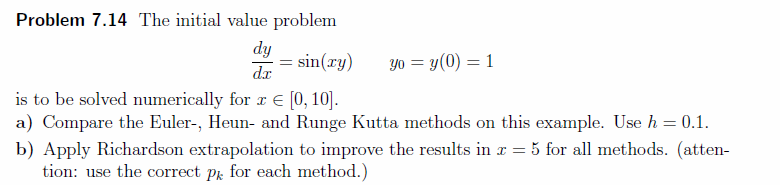
\includegraphics[width=1\textwidth]{chapters/images/desc-7-14}
%\end{figure}


\subsubsection{a)}

To calculate the respective $y$ values we can simply use the functions from Problem 7.13:

\begin{lstlisting}[caption=Problem 7.14 a)]
def myF(x, y):
	return math.sin(x * y);

xses = [];

for i in range(102): xses.append(i / 10.0);

eulerYses = dif.euler(myF, 0, 10, 1, 0.1);
heunYses = dif.heun(myF, 0, 10, 1, 0.1);
rungeKuttaYses = dif.rungeKutta(myF, 0, 10, 1, 0.1);

plt.plot(xses, eulerYses);
plt.plot(xses, heunYses);
plt.plot(xses, rungeKuttaYses);
plt.xlabel("x");
plt.ylabel("y");
plt.show();
\end{lstlisting}

The resulting graph of each method looks like the following:

\newpage

\begin{figure}[!ht]
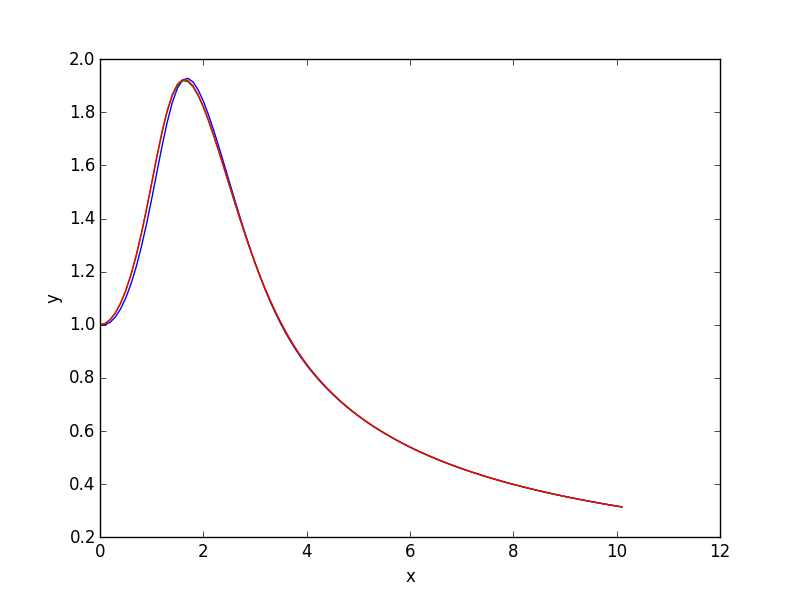
\includegraphics[width=1\textwidth]{chapters/images/figure-7-14-a}
\caption{Graph of the results of the 3 methods}
\end{figure}

As it can be seen, the graphs of the functions are very close to each other and there is hardly any difference noticeable.

\subsubsection{b)}

Again, using the functions from Problem 7.13 we can simply calculate the $y$ values with the Richardson extrapolation:

\begin{lstlisting}[caption=Problem 7.14 b)]
eulerRichardsonYses = dif.eulerRichardson(myF, 0, 10, 1, 0.1);
heunRichardsonYses = dif.heunRichardson(myF, 0, 10, 1, 0.1);
rungeKuttaRichardsonYses = dif.rungeKuttaRichardson(myF, 0, 10, 1, 0.1);

print("euler: " + str(eulerRichardsonYses[50]));
print("heun: " + str(heunRichardsonYses[50]));
print("runge-kutta: " + str(rungeKuttaRichardsonYses[50]));
\end{lstlisting}

The result of these calculations are:

\begin{lstlisting}[caption=Result of 7.14 b), keywordstyle=\color{black}]
euler: 0.656662162824
heun: 0.657837825456
runge-kutta: 0.657541150858
\end{lstlisting}

As expected, the value approximated with Euler's method is slightly below the other method's values, however with the Richardson extrapolation this error is not as critical as it would have been if the regular methods had been used.


\subsection{Problem 7.15}


\begin{figure}[!ht]
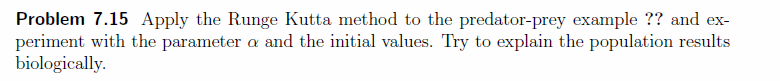
\includegraphics[width=1\textwidth]{chapters/images/desc-7-15}
\end{figure}

To simulate the predator-prey-model an ODE system has to be created, with one equation for the sheep and one for the wolfs. Afterwards, the solution can be simply calculated with the script from Problem 7.13:

\begin{lstlisting}[caption=Problem 7.15]
def sheepFunc(t, yVector):
	return 10 * yVector[0] * (1 - yVector[1]);

def wolfsFunc(t, yVector):
	return yVector[1] * (yVector[0] - 1);

fses = [];
y0ses = [];

fses.append(sheepFunc);
fses.append(wolfsFunc);
y0ses.append(3);
y0ses.append(1);

yVectors = dif.rungeKuttaSystem(fses, 0, 5, y0ses, 0.05);

xses = [];
sheepYses = [];
wolfsYses = [];

x = 0;

for yVector in yVectors:
	sheepYses.append(yVector[0]);
	wolfsYses.append(yVector[1]);
	xses.append(x);
	x += 0.05;

plt.plot(xses, sheepYses);
plt.plot(xses, wolfsYses);
plt.xlabel("x");
plt.ylabel("y");
plt.show();
\end{lstlisting}

Depending on $\alpha$ and the initial number of sheep and wolfs the graphs look like this:

\begin{figure}[!ht]
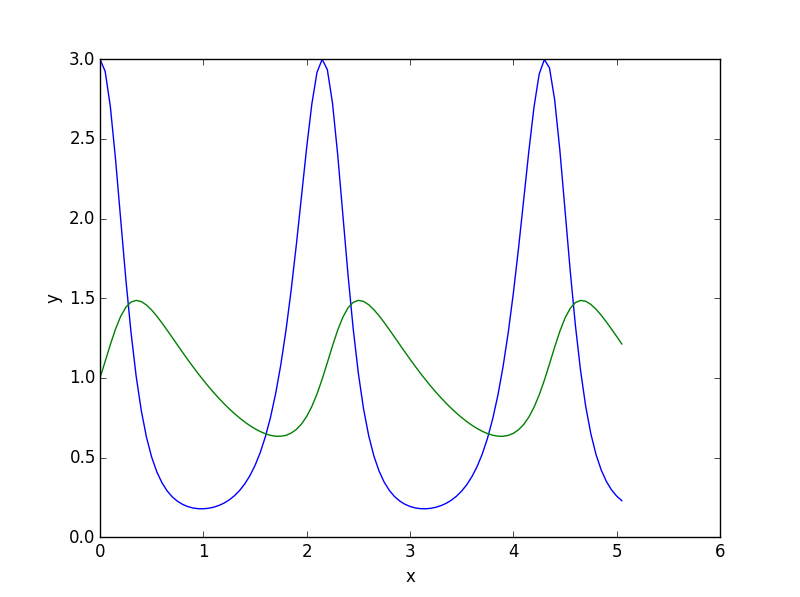
\includegraphics[width=1\textwidth]{chapters/images/figure-7-15-1}
\caption{$\alpha = 10$, initially 3 sheep and 1 wolfs}
\end{figure}

\begin{figure}[!ht]
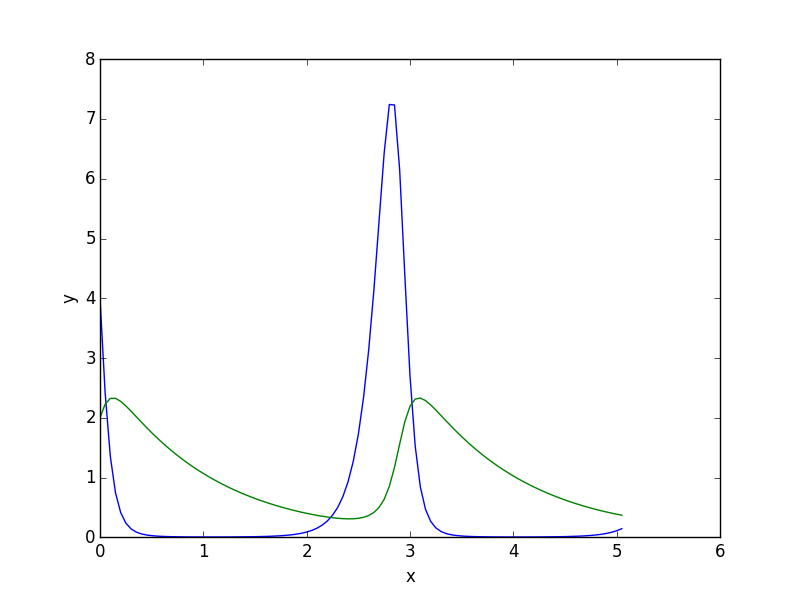
\includegraphics[width=1\textwidth]{chapters/images/figure-7-15-2}
\caption{$\alpha = 9$, initially 4 sheep and 2 wolfs}
\end{figure}

\begin{figure}[!ht]
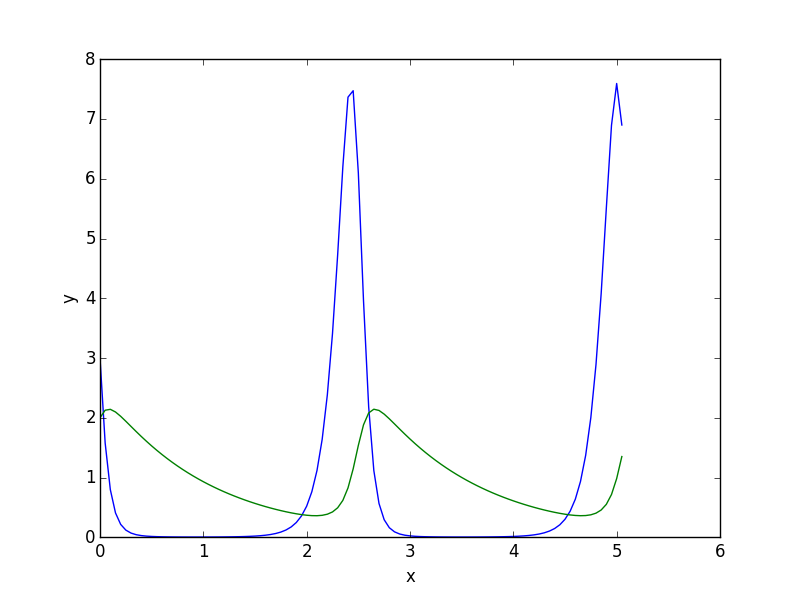
\includegraphics[width=1\textwidth]{chapters/images/figure-7-15-3}
\caption{$\alpha = 12$, initially 3 sheep and 2 wolfs}
\end{figure}

Biologically, this could be explained by the balance between predator and prey which is mandatory for both species to survive.


\newpage

\subsection{Problem 7.16}

\begin{figure}[!ht]
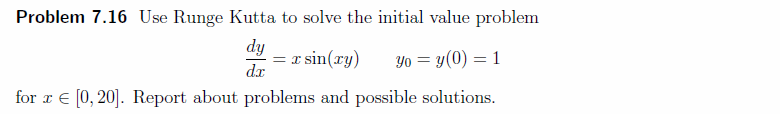
\includegraphics[width=1\textwidth]{chapters/images/desc-7-16}
\end{figure}

\begin{lstlisting}[caption=Problem 7.16]
def myF(x, y):
	return x * math.sin(x * y);

xses = [];

for i in range(201): xses.append(i / 10.0);

yses = dif.rungeKutta(myF, 0, 20, 1, 0.1);

plt.plot(xses, yses);
plt.xlabel("x");
plt.ylabel("y");
plt.show();
\end{lstlisting}

The resulting graph looks like:

\begin{figure}[!ht]
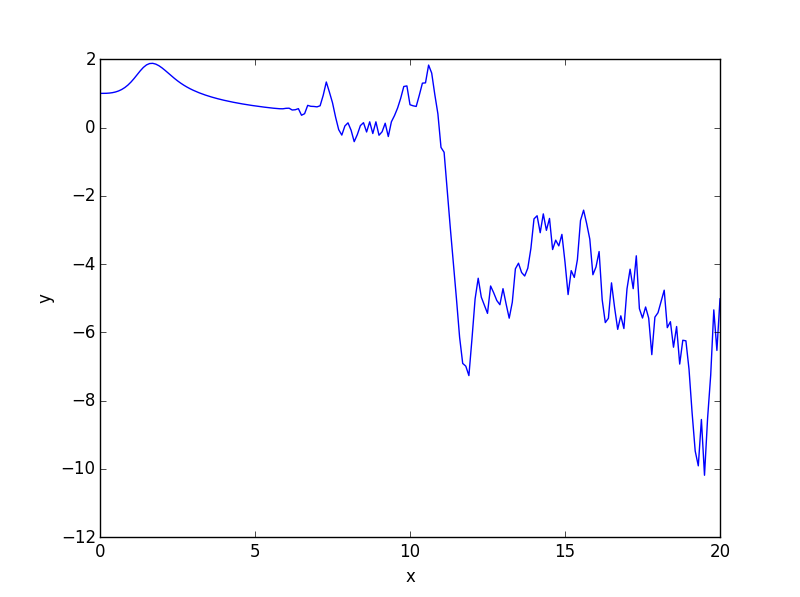
\includegraphics[width=1\textwidth]{chapters/images/figure-7-16}
\caption{Graph of Problem 7.16}
\end{figure}


Since the $x$ parameter is a factor both inside and outside of the sine, the frequency as well as the amplitude increase as $x$ grows. Hence, the fluctuation increases and the slopes get steeper and steeper. Because the step size stays the same, the curve gets \enquote{spikier} and slightly inaccurate. A possible solution could be to decrease the step size.





\end{document}